\documentclass[14pt]{beamer}
\usetheme{Boadilla}
\usecolortheme{whale}
\setbeamertemplate{navigation symbols}{}
\usepackage{comment}

%\usepackage{ctex}

%\setbeamertemplate{theorems}[numbered]

\usepackage{textcomp}
\usepackage{float}
\usepackage{multirow}
\usepackage{comment}
\usepackage{enumitem}
\usepackage{tikz}
\usepackage{algorithm}
\usepackage{adjustbox}
\usepackage{epstopdf}
\usetikzlibrary{arrows,decorations,shapes}
\usepackage{amsmath}
\usepackage{multicol}
\usepackage{threeparttable}
\usepackage{mathrsfs}
\usepackage{arydshln}

%\usepackage[UTF8, heading = false, scheme = plain]{ctex}


\usepackage{amsfonts,amsthm,amssymb,amsmath}
\usepackage{graphicx,mathrsfs}
\usepackage{adjustbox}
\usepackage{multirow}
\usepackage{float}
\usepackage{hyperref}
\usepackage{tikz}
\usetikzlibrary{backgrounds}
\usepackage{algorithm}
%\usetikzlibrary{snakes}
\usepackage{subfig}
\usepackage{ragged2e}
\usepackage{framed}
\usepackage{multicol}
\definecolor{shadecolor}{rgb}{0.9,0.9,0.9}

\setbeamerfont{frametitle}{size=\large}


% Setup appearance:


\newcommand{\labelitemi}{$\bullet$}
\newcommand{\BM}{\mathcal{B}} % Brownian motion
\newcommand{\cl}[1]{\lceil{#1}\rceil} % ceiling of a number
\newcommand{\R}{\mathbb{R}}
\newcommand{\Z}{\mathbb{Z}}
\newcommand{\cc}{\mathbb{c}}



% Author, Title, etc.

\title[Grand Coalition Stabilization]
{%
{
Stabilizing Grand Cooperation in Unbalanced Cooperative Games%
}
}

\author[{\color{olive}{\bf Xiangtong Qi}}] % (optional, use only with lots of authors)
%{F.~Author\inst{1} \and S.~Another\inst{2}}
{   %  \textit{Supervisor:}
  Xiangtong Qi
}
\date
{MISTA, Ningbo, Dec. 2019}

\institute[] % (optional, but mostly needed)
{\footnotesize
	Department of Industrial Engineering and Decision Analytics,\\
\vspace{2mm}
	The Hong Kong University of Science and Technology\\
    \vspace{5mm}
	Joint works with {\color{olive}{\bf Lindong Liu}} (USTC), {\color{olive}{\bf Zhou Xu}} (HKPU)
	\vspace{3mm}
}



% The main document


\begin{document}

\begin{frame}
  \titlepage
\end{frame}


%\begin{frame}{Outline}
%\tableofcontents
%\end{frame}

\section{Introduction}
\begin{frame}
\centering
\large
\textcolor{blue}{\bf {\huge I}NTRODUCTION}
\end{frame}
%\subsection{Supply Chain and Cooperation}
\begin{frame}{Cooperation}
\justifying
\textcolor{red}{\bf Cooperation} is everywhere, from cells in your body, to people in a city, and partners in \textcolor{red}{\bf a scheduling problem}.\\
~\\
\pause
\vspace{3mm}
\begin{itemize}
\justifying
	\color{blue}
	\item centralized decision making, to minimize the total cost (for social optimum);\\
	\item enforced by an external party, to minimize negative externalities (e.g. the number of machines used, etc).
\end{itemize}
\end{frame}


\begin{frame}{Cooperation}
\justifying
\centering
Is every player beneficial from the grand cooperation?\\
\vspace{3mm}
Is the grand cooperation stable? \\
~\\
	\pause
	\centering
\textcolor{red}{Not Always.}\\
\vspace{3mm}
\textcolor{red}{If the grand cooperation is not stable, how to stabilize it?}
\end{frame}

\section{Preliminaries}
\begin{frame}
\centering
\large
\textcolor{blue}{\bf {\huge P}RELIMINARIES}
\end{frame}
%\subsection{Supply Chain and Cooperation}
%\subsection{Stabilizing the Cooperation}
\begin{frame}{Cooperative Game}
A \textcolor{red}{\bf  cooperative game} is defined by a pair $(N,\pi)$:
\begin{itemize}
\justifying
	\item A set $N = \big\{1,2,\ldots,n\big\}$ of players, \textcolor{red}{\bf grand colaition};
%	\item $S = 2^V \setminus \{\emptyset\}$: set of all non-empty coalitions
	\item A \textcolor{red}{\bf characteristic function} $\pi(S)$ = the minimum total cost achieved by the cooperation of members in coalition $S \in \mathbb{S}=2^N \setminus \{\emptyset\}$.
\end{itemize}

~\\The game requires:
\begin{itemize}
\justifying
	\item A \textcolor{red}{\bf cost allocation} $\alpha=\big[\alpha_1,\alpha_2,\ldots,\alpha_n \big] \in \R^n$, where $\alpha_j$ = the cost allocated to each player $j \in N$.
\end{itemize}
\end{frame}


\begin{frame}{Integer Minimization Games}
\justifying
\small
\vspace{-2mm}
\begin{shaded}
\centering
$\pi(S)$: need to solve an optimization problem, not given.
\end{shaded}

\textcolor{red}{\bf Integer Minimization (IM) Games:}\\
~\\
For each coalition $S \in \mathbb{S}$, an incidence vector $y^S \in \{0,1\}^{n}$, with $y_j^S=1$ if $j \in S$, and with $y_j^S=0$ otherwise, for all $j \in N$, such that
\begin{equation*}
\color{blue}
\pi(S) = \min_{x} \{ cx: Ax \geq By^S + E, ~x \in \Z^{q} \}.
\end{equation*}
\end{frame}

\begin{frame}{Core}
\small
Denote $\alpha(S)=\sum_{j \in S}\alpha_j$. \\~\\
A cost allocation $\alpha \in \R^n$ is in the \textcolor{red}{\bf core} if it satisfies:
\begin{itemize}
\small
\justifying
	\item \textcolor{red}{\bf Budget Balance} Constraint: $\alpha(N)=\pi(N)$;
	\item \textcolor{red}{\bf Coalition Stability} Constraints: $\alpha(S)\leq \pi(S)$ for each  $S\in \mathbb{S}$.
\end{itemize}
%\pause
\vspace{-12pt}
\begin{eqnarray*}
\mathrm{Core}(N,\pi) = &&\bigg\{ \alpha:~ \alpha(N)=\pi(N), \\
&& \alpha(S) \leq \pi(S), ~\forall S \in \mathbb{S} \setminus \{N\},~\alpha \in \R^n   \bigg\}.
\end{eqnarray*}

\pause
\vspace{-12pt}
\textcolor{cyan}{However, $\mathrm{Core}(N,\pi)$ can be empty.}
\end{frame}


\begin{frame}{Example: Machine Scheduling Game (MSG)}
\small
%\begin{example}[SMW Game]
\textcolor{blue}{Game of Single Machine Scheduling with Setup Cost:}
\vspace{2mm}
	\begin{itemize}
	\justifying
		\item Grand coalition: $N = \big\{ 1,2,3,4 \big\}$;
		\item Processing times: $t_1=2$, $t_2=3$, $t_3=4$, $t_4=5$;
		\item Machine setup cost: $t_0 = 9.5$;
		\item $\pi(S)$ for $S\in \mathbb{S}$:  minimizes the total completion time of jobs in $S$ plus the machine setup cost;
		\item \textcolor{red}{$\pi(N)= \pi(\{1,3\}) + \pi(\{2,4\})= 38$ (SPT Rule).}

\vspace{6pt}
%\begin{center}
{
\centering
\scalebox{0.8}{
\begin{tikzpicture}[x=1cm,y=1.5cm,scale=0.8]
% draw horizontal line
\draw (0,0) -- (6,0);

\draw (8,0) -- (16,0);

% draw vertical lines
%\def\vectime{{0,5,11,18,26}}
%\def\vectimeb{{0,2.5,8,14.5,22}}
\foreach[count=\i] \x in {0,2,6}
{
	\draw (\x,3pt) -- (\x,-3pt);
	\draw (\x,0) node[below=3pt] {$\x$} node[above=3pt] {$   $};
%	\draw (\vectime[\i],3pt) -- (\vectime[\i],-3pt);
%	\x = \vectime[\i];
%	\draw (\vectime[\i],0) node[below=3pt] {$\x$} node[above=3pt] {$   $};
}
\foreach[count=\i] \x in {0,3,8}
{
	\draw (\x+8,3pt) -- (\x+8,-3pt);
	\draw (\x+8,0) node[below=3pt] {$\x$} node[above=3pt] {$   $};
%	\draw (\vectime[\i],3pt) -- (\vectime[\i],-3pt);
%	\x = \vectime[\i];
%	\draw (\vectime[\i],0) node[below=3pt] {$\x$} node[above=3pt] {$   $};
}

\draw (1,0) node[above=3pt] {job 1};
\draw (4,0) node[above=3pt] {job 3};
\draw (10,0) node[above=3pt] {job 2};
\draw (13,0) node[above=3pt] {job 4};

\end{tikzpicture}
}
\par
}
%\pause

\end{itemize}
\end{frame}


\begin{frame}{Example: Empty Core}
\small
\vspace{-4mm}
\begin{columns}
\begin{column}{4.5cm}
\begin{table}[H]
\centering
\tabcolsep=8pt
\footnotesize
\renewcommand\arraystretch{1.1}
%\caption{\label{table:examplecost} Coalitional cost}
\vglue5pt
\vspace{-3mm}
\begin{tabular}[!h]{c c }
\hline
\multicolumn{1}{c}{Coalitions} &\multicolumn{1}{c}{Cost}\\
\hline
$\{1\}$		&11.5	\\

$\{2\}$		&12.5	\\

$\{3\}$		&13.5	\\

$\{4\}$		&14.5  \\

$\{1,2\}$		&16.5	\\

$\{1,3\}$		&17.5	\\

$\{1,4\}$		&18.5	\\

$\{2,3\}$		&19.5	\\

$\{2,4\}$		&20.5	\\

$\{3,4\}$		&22.5	\\

$\{1,2,3\}$		&25.5	\\

$\{1,2,4\}$		&26.5	\\

$\{1,3,4\}$		&28.5	\\

$\{2,3,4\}$		&31.5	\\

\textcolor{blue}{$\{1,2,3,4\}$}	&\textcolor{blue}{38}	\\
\hline
\end{tabular}
\end{table}
\end{column}
\pause
\begin{column}{6.5cm}
\footnotesize
\vspace{-1em}
\begin{shaded}
\centering
Optimal Cost Allocation Problem
\begin{eqnarray*}
\begin{aligned}
\max ~\big(\alpha_1 + \alpha_2 + \alpha_3 + \alpha_4\big) &= \textcolor{red}{37.25 < 38}\\
s.t.~~ \alpha_1 \leq 11.5,~\cdots,&~\alpha_4 \leq 14.5,\\
\alpha_1 + \alpha_2 \leq 16.5,~\cdots,~ &\alpha_3+\alpha_4 \leq 22.5,\\
~~~~~~~~~~\cdots,~~&\\
\alpha_1 + \alpha_2 + \alpha_3 + \alpha_4 &\leq 38.
\end{aligned}
\end{eqnarray*}
\vspace{-0.5em}
\end{shaded}
\begin{shaded}
\centering
\textcolor{blue}{
$\alpha^* = \big[6;8.75;10.75;11.75\big]$}
\end{shaded}
\end{column}
\end{columns}
\end{frame}



\section{Instruments}
\begin{frame}
\centering
\large
\textcolor{blue}{\bf {\huge I}NSTRUMENTS}
\end{frame}

\begin{frame}{Instruments to Stabilize Grand Coalitions}
\begin{figure}[H]
\centering
\begin{minipage}[t]{0.32\textwidth}
\centering

\includegraphics[width=0.7\textwidth]{conculsion1.png}
\captionsetup{font={scriptsize}}
\caption*{Unbalanced Game}
\end{minipage}
\begin{minipage}[t]{0.32\textwidth}
\centering
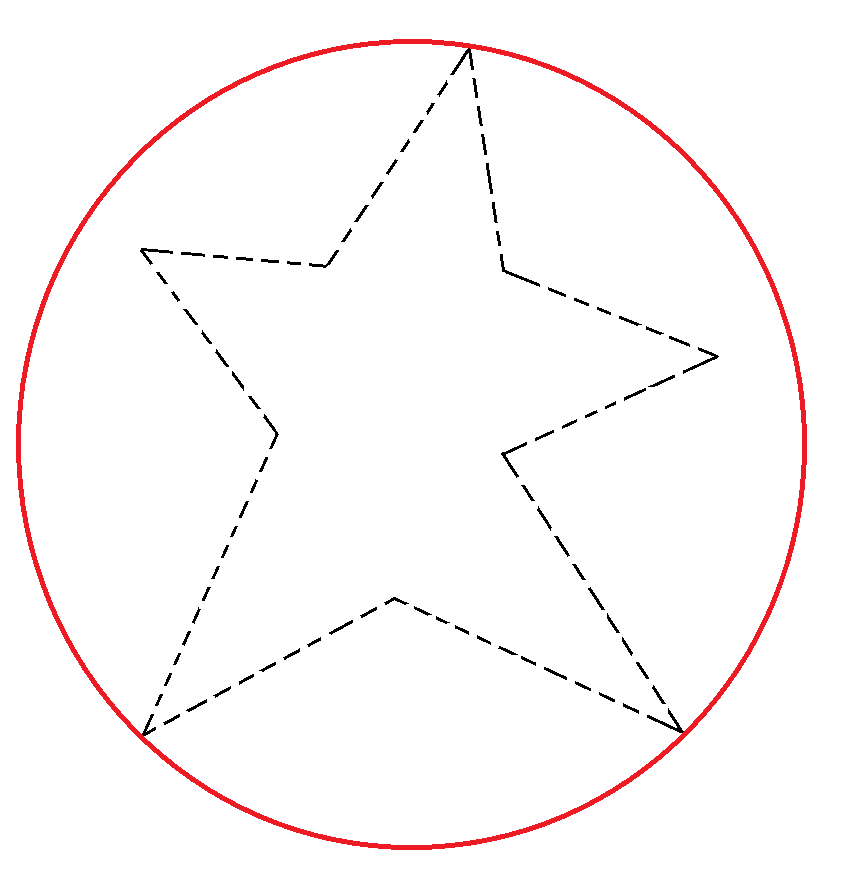
\includegraphics[width=0.82\textwidth]{conculsion3.png}
\captionsetup{font={scriptsize}}
\caption*{Subsidization}
\end{minipage}
\begin{minipage}[t]{0.32\textwidth}
\centering
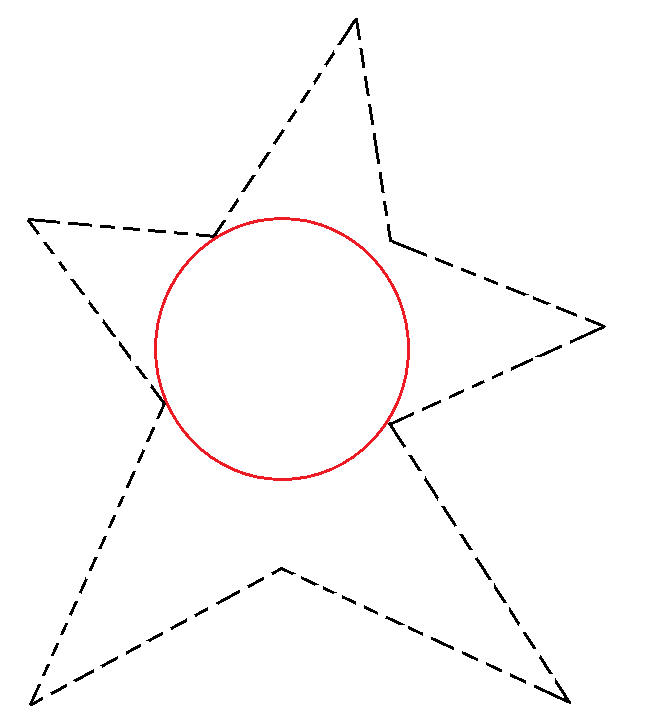
\includegraphics[width=0.7\textwidth]{conculsion2.png}
\captionsetup{font={scriptsize}}
\caption*{Penalization}
\end{minipage}
\end{figure}
\begin{figure}[H]
\centering
\begin{minipage}[t]{0.49\textwidth}
\centering
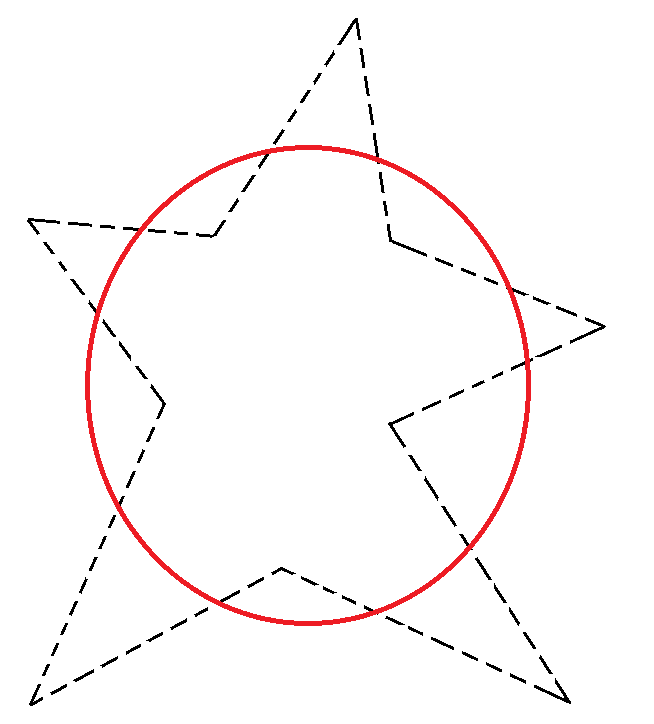
\includegraphics[width=0.42\textwidth]{conculsion4.png}
\captionsetup{font={scriptsize}}
\caption*{Simultaneous Subsidization \& Penalization}
\end{minipage}
\begin{minipage}[t]{0.49\textwidth}
\centering
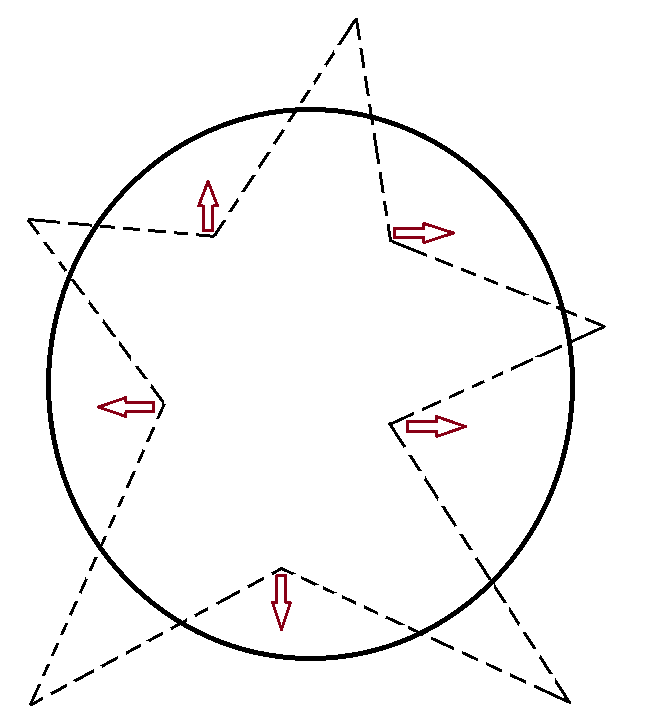
\includegraphics[width=0.42\textwidth]{conculsion5.png}
\captionsetup{font={scriptsize}}
\caption*{Cost Adjustment}
\end{minipage}
\end{figure}
\end{frame}



\begin{frame}{Our Studies}
\begin{table}[t]
	\small
	\centering
	\tabcolsep=5pt
	%\small
	\renewcommand\arraystretch{1.8}
	%\caption{\label{table:example1}$z$-penalized minimum subsidies for the example.} % under different penalties}
	\vglue5pt
	\vspace{-3mm}
	\begin{tabular}[!h]{c c}
		\hline
		\textcolor{red}{\bf S.}	&Caprara and Letchford (2010, MP), \textcolor{blue}{Liu et al. (2016, IJOC)}\\
		\textcolor{red}{\bf P.}	&Schulz and Uhan (2010, OR; 2013, DO)\\
		\textcolor{red}{\bf P.\&S.}	&\textcolor{blue}{Liu et al. (2018, OR)}\\
		\textcolor{red}{\bf C.A.}	&\textcolor{blue}{Liu et al. (2019, under review)}\\
		\hline
	\end{tabular}
	\vspace{-3mm}
	%c(N)=115
\end{table}
\end{frame}



\subsection{Instrument of Subsidization}
\begin{frame}
\centering
\normalsize
\textcolor{olive}{\bf {\LARGE 1.} \bf {\LARGE I}NSTRUMENT OF {\bf {\LARGE S}}UBSIDIZATION}
\vspace{5mm}
\begin{figure}[H]
\centering
\begin{minipage}[t]{0.32\textwidth}
\centering

\includegraphics[width=0.5\textwidth]{conculsion1.png}
\captionsetup{font={scriptsize}}
\caption*{Unbalanced Game}
\end{minipage}
\begin{minipage}[t]{0.32\textwidth}
\centering
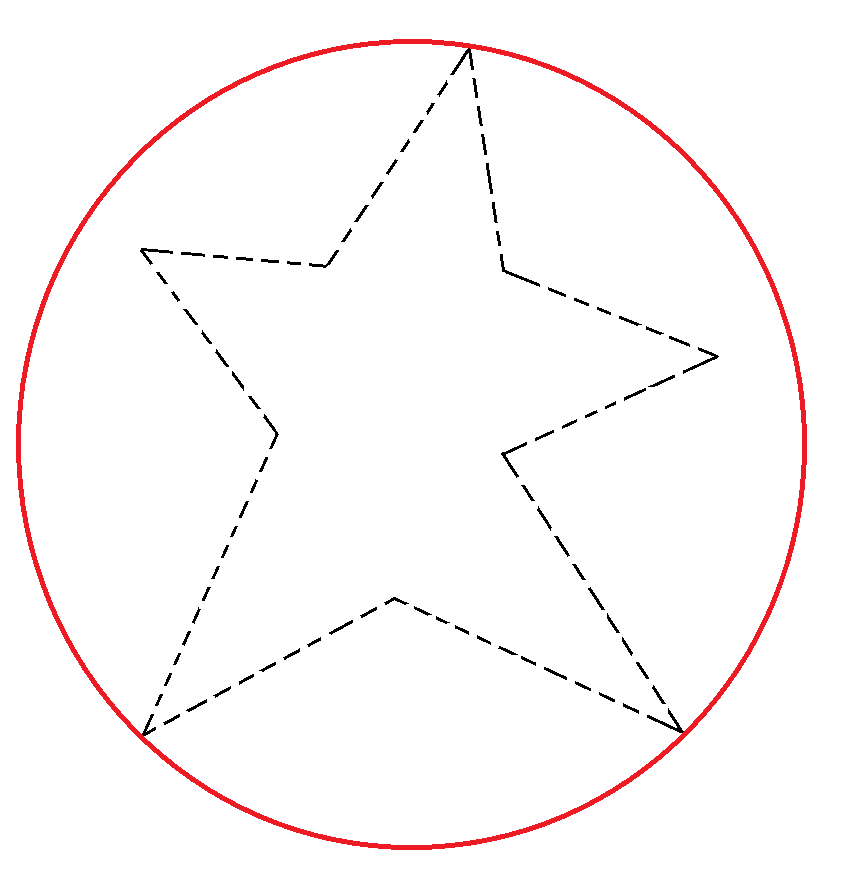
\includegraphics[width=0.6\textwidth]{conculsion3.png}
\captionsetup{font={scriptsize}}
\caption*{Subsidization}
\end{minipage}
\end{figure}
\vspace{-15mm}
\end{frame}

\begin{frame}{Instrument 1: LRB Cost Allocation, {\footnotesize 2016, IJOC}}{Instrument of Subsidization ($\epsilon$-core)}
\vspace{3mm}
{\footnotesize $\mathrm{Core}(N,\pi) = \bigg\{ \alpha:~ \alpha(N)=\pi(N), ~\alpha(S) \leq \pi(S), ~\forall S \in \mathbb{S} \setminus \{N\},~\alpha \in \R^n   \bigg\}$.}

\begin{shaded}
\centering \textcolor{red}{\bf Relax Budget Balanced constraint}: $\alpha(N) = \pi(N)$
\end{shaded}
\begin{itemize}
\item \textcolor{blue}{Minimum Subsidy} to stabilize the grand coalition:
\begin{equation*}
\omega^* = \min \big\{ \pi(N) - \alpha(N): \alpha(S) \leq \pi(S), ~\forall S \in \mathbb{S} \big\}.
\end{equation*}
\end{itemize}
\pause
\vspace{-7mm}
\begin{shaded}
\centering
\small
Minimum Subsidy needed for MSG Example:\\
\vspace{2mm}
\textcolor{red}{$\omega^*=38-37.25 = 0.75$}
\end{shaded}
\end{frame}


\begin{frame}{Instrument 1: LRB Cost Allocation, {\footnotesize 2016, IJOC}}{Linear Programming Relaxation Based (LPB) Cost Allocation Method}
\vspace{-5mm}
\small
\begin{shaded}
\centering
{\bf Optimal Cost Allocation Problem (OCAP)}:
\begin{equation*}
\max_{\alpha}\big\{ \alpha(N):\alpha(S) \leq \pi(S), ~\forall S \in \mathbb{S} \big\}.
\end{equation*}
\vspace{-2em}
\end{shaded}

\textcolor{red}{\bf \centerline{All existing methods are based on Linear Relaxation}}\\
\vspace{-3mm}
\begin{shaded}
\vspace{-6mm}
\footnotesize
\begin{eqnarray*}
f(x) = cx ~\Longrightarrow~ \pi(S) = \min_{x} \big\{ cx:~Ax \geq B\gamma^s + E, ~A'x \geq B'\gamma^s + E', ~x \in \{0,1\}^{q} \big\}
\end{eqnarray*}
\vspace{-8mm}
\end{shaded}
\vspace{-5mm}
\setbeamersize{description width=1cm}
\begin{description}
\justifying
\footnotesize
	\item[Step 1.] \textcolor{red}{Find an LP $\min_x \big\{cx:Gx \geq F\gamma^s\big\}$} giving a \textcolor{red}{lower bound $\pi_{\mathrm{LP}}(S)$ to $\pi(S)$};
	\item[Step 2.] \textcolor{red}{Compute $\big(\alpha^{GF}_{LP}\big)_j = \big(\mu^*\big)^T F_{\cdot j}$}, where $\mu^*$: dual solution; $F_{\cdot j}$: $j$-th column.
	\item[Step 3.] \textcolor{red}{Obtain an LPB cost allocation $\alpha^{GF}_{LP}$} with \textcolor{red}{$\alpha^{GF}_{LP}(N) = \pi_{\mathrm{LP}}(N)$}.
\end{description}



%\begin{shaded}
%\centering
%LPB v.s. LRB Cost Allocation Methods\\
%(Caprara and Letchford, 2010, Mathematical Programming)
%\end{shaded}
%\vspace{-5mm}
%\begin{columns}
%\begin{column}{7cm}
%\begin{itemize}
%\footnotesize
%\item Decide assignable constraints set;
%\item Solve the LP dual variables;
%\item Compute LPB cost allocation.
%\end{itemize}
%\end{column}
%\begin{column}{7cm}
%\begin{itemize}
%\footnotesize
%\item Not general to implement;
%\item Not very effective;
%\item Only suitable for linear $f(x)$.
%\end{itemize}
%\end{column}
%\end{columns}
\end{frame}



\begin{frame}{Instrument 1: LRB Cost Allocation, {\footnotesize 2016, IJOC}}{Research Questions}
\vspace{-5mm}
\begin{shaded}
\centering
Lagrangian Relaxation v.s. Linear Relaxation
\end{shaded}
\vspace{-5mm}
\begin{columns}
\begin{column}{5.5cm}
\begin{itemize}
\footnotesize
\item Applicable in non-linear case;
\item Generally more effective;
\end{itemize}
\end{column}
\begin{column}{8cm}
\begin{itemize}
\footnotesize
\item New insights via decomposition;
\item Adequate studies on LR for ILP.
\end{itemize}
\end{column}
\end{columns}
\begin{shaded}
\small
\textcolor{red}{\bf Compute a cost allocation} based on \textcolor{red}{\bf Lagrangian Relaxation} technique such that
\begin{itemize}
\item  the cost assigned to each coalition \textcolor{red}{\bf  does not exceed the total cost incurred} if they deviate from grand coalition;
\item the total assigned cost is \textcolor{red}{\bf as large as possible}.
\end{itemize}
\vspace{-2mm}
\end{shaded}
\end{frame}




\begin{frame}{Instrument 1: LRB Cost Allocation, {\footnotesize 2016, IJOC}}{Lagrangian Relaxation, Lagrangian Decomposition, Sub-games Analyses}
\footnotesize
\vspace{-7mm}
\begin{shaded}
\vspace{-1mm}
\begin{equation*}\label{eqn:orgc}
\textcolor{blue}{\pi(S)} = \min_{x} \big\{ f(x):Ax \geq B\gamma^s + E, ~A'x \geq B'\gamma^s + E', ~x \in \{0,1\}^{q} \big\}
\end{equation*}
\vspace{-5mm}
\end{shaded}
\vspace{-5mm}
\begin{itemize}
\footnotesize
\item  \textcolor{red}{\bf Lagrangian characteristic function}, $\forall S \in \mathbb{S}$:
\begin{eqnarray*}
\textcolor{blue}{\pi_{LR}^{\lambda}(S)} = \min_{x}  \{f(x)-\lambda (A'x - B'\gamma^s - E'):
       Ax \geq B\gamma^s + E, x \in \{0,1\}^{q \times 1}\}.
\end{eqnarray*}
\vspace{-6mm}
\item \textcolor{red}{\bf Lagrangian sub-characteristic functions 1 and 2}, $\forall S \in \mathbb{S}$:
\begin{eqnarray*}\label{eqn:subcf1}
\begin{aligned}
\textcolor{blue}{\pi_{LR1}^{\lambda}(S)} = \lambda  B'\gamma^s + \lambda E', ~\forall S \in \mathbb{S}.
\end{aligned}
\end{eqnarray*}
\vspace{-8mm}
\begin{eqnarray*}
\textcolor{blue}{\pi_{LR2}^{\lambda}(S)} = \min_x \{ f(x)-\lambda A'x: Ax \geq B\gamma^s + E, ~x \in \{0,1\}^{q} \}, ~\forall S \in \mathbb{S}.
\end{eqnarray*}
\vspace{-1.8em}
\item \textcolor{red}{\bf Sub-games 1 and 2}:
\begin{itemize}
\justifying
\item[$-$] Sub-game 1, vector $\textcolor{blue}{(\alpha_{LR1}^{\lambda})_j} = (\lambda B')_j + \frac{1}{n}\lambda E',~\forall j \in N$, in the core;\\
\vspace{2mm}
\item[$-$] Sub-game 2, optimal cost allocation $\textcolor{blue}{\alpha_{LR2}^{\lambda}}$: Primal-Dual-Type alg. (sub-modular), Column Generation Based alg. (not sub-modular).
\end{itemize}
\end{itemize}
\end{frame}


\begin{frame}{Instrument 1: LRB Cost Allocation, {\footnotesize 2016, IJOC}}{LRB Cost Allocation}
\footnotesize
\begin{theorem}\label{thm:lrcostallocationfeasible}
\justifying
\rm{
Given any Lagrangian multiplier $\lambda$, \textcolor{red}{if $\alpha_{LR1}^{\lambda}$ and $\alpha_{LR2}^{\lambda}$ are feasible} cost allocations for sub-games $(N,\pi_{LR1}^{\lambda})$ and $(N,\pi_{LR2}^{\lambda})$, respectively,\\
\vspace{3mm}
~~~~then \textcolor{red}{$\alpha_{LR}^{\lambda} = \alpha_{LR1}^{\lambda} + \alpha_{LR2}^{\lambda}$ is a feasible} cost allocation for game $(N,\pi)$.}
\end{theorem}
\vspace{-0.1cm}
\begin{theorem}\label{thm:lagcostallocation1}
\rm
For game $(N,\pi)$, under the same ILP formulation for $\pi(S)$, the LRB cost allocation value is no less than the LPB cost allocation value, i.e., $\alpha_{LR}^{\lambda}(N) \geq \alpha_{LP}(N)$, when
\begin{itemize}
\item[(1)] \textcolor{red}{Given Lagrangian multiplier is optimal, i.e., $\lambda = \lambda^*$;}
\item[(2)] \textcolor{red}{$Core(N,\pi_{LR2}^{\lambda})$ is non-empty.}
\end{itemize}
\end{theorem}
\end{frame}




\begin{frame}{Instrument 1: LRB Cost Allocation, {\footnotesize 2016, IJOC}}{Applications of the LRB Cost Allocation Method}
\small
\begin{shaded}
\centering
Applications on Four Types of Facility Location Games
\end{shaded}
\begin{table}[H]
\centering
\tabcolsep=2pt
\footnotesize
\renewcommand\arraystretch{2}
\begin{tabular}[!h]{c| c c| c}

\multicolumn{1}{c|}{} &\multicolumn{1}{c}{Sub-modular} & \multicolumn{1}{c}{Not Sub-modular}& \multicolumn{1}{|c}{Applicable Method(s)}\\
\hline
Linear	&Type one: UFL	&Type two: CFL	&\textcolor{red}{LPB, LRB}\\

Non-linear	&Type three: NLUFL	&Type four: NLCFL	&\textcolor{red}{LRB}\\
\end{tabular}
\end{table}

\end{frame}


\begin{frame}{Instrument 1: LRB Cost Allocation, {\footnotesize 2016, IJOC}}{Uncapacitated Facility Location Game}
\small
\centering
\begin{theorem}
\justifying
\small
\centering
\textbf{\rm LRB cost allocation and LPB cost allocation are both optimal.}
\end{theorem}
\begin{shaded}
\footnotesize
\centering
The optimal cost allocations computed by different methods for the example
\end{shaded}
\vspace{-0.1em}
\scriptsize
\renewcommand\arraystretch{1.4}
\begin{tabular}[!h]{c c c c c c c c}
\hline
\multicolumn{1}{c}{Method} &\multicolumn{1}{c}{Player 1}&\multicolumn{1}{c}{Player 2} &\multicolumn{1}{c}{Player 3}  &\multicolumn{1}{c}{Player 4} &\multicolumn{1}{c}{Total}\\
\hline
LPB with Simplex	&5.00	&6.50	&8.50	&6.50	&\textcolor{teal}{\bf 26.5}	&\\
LPB with Interior Point	&6.58	&6.50	&8.50	&4.92	&\textcolor{teal}{\bf 26.5}	&\\
LRB	&6.87	&6.50	&8.50	&4.63	&\textcolor{teal}{\bf 26.5}	&\\
\hline
\end{tabular}
\vspace{0.5em}
\begin{shaded}
\vspace{-0.8em}
\begin{itemize}
\justifying
\footnotesize
\item LRB cost allocation \textcolor{red}{shares the same amount of cost} as LPB cost allocation, in addition, LRB algorithm can sometimes generate cost allocations which are \textcolor{red}{not easy to obtain by conventional LPB methods}.
\end{itemize}
\vspace{-1.2em}
\end{shaded}
\end{frame}



\begin{frame}{Instrument 1: LRB Cost Allocation, {\footnotesize 2016, IJOC}}{Single Source Capacitated Facility Location Game}
\footnotesize
\begin{table}[H]
\centering
\tabcolsep=5pt
\footnotesize
\renewcommand\arraystretch{1.3}
%\caption{\label{table:LRBLPBSG}LPB vs. LRB cost allocations in CFL}
\setlength{\abovecaptionskip}{100pt}
\setlength{\belowcaptionskip}{100pt}
\vglue2pt
\begin{tabular}[!h]{c c c c c c c c c c c c c c}
\hline
\multirow{2}{*}{Q} &\multicolumn{2}{c}{} & \multicolumn{2}{c}{Average (\%)}  &\multicolumn{2}{c}{} &\multicolumn{2}{c}{LRCA - LPCA (\%)} &\multicolumn{2}{c}{} &\multicolumn{3}{c}{Total time (s)}\\
\cline{4-5}
\cline{8-9}
\cline{12-14}
& && LPCA & LRCA	&& &Max	&Min	&& &Avg. &Max	&Min\\
\hline
10  &&  &{\color{teal}{\bf 97.15}}	&{\color{blue}{\bf 98.79}}	&&	&2.38	&1.00	&&	&19	&21	&18\\

20  &&  &{\color{teal}{\bf 97.20}}	&{\color{blue}{\bf 98.31}}	&&	&1.51	&0.88	&&	&24	&27	&23\\

30  &&  &{\color{teal}{\bf 94.70}}	&{\color{blue}{\bf 95.25}}	&&	&0.75	&0.38	&&	&15 &28	&21\\

40  &&  &{\color{teal}{\bf 94.11}}	&{\color{blue}{\bf 94.25}}	&&	&0.28	&0.07	&&	&24	&24	&23\\

50  &&  &{\color{teal}{\bf 93.87}}	&{\color{blue}{\bf 93.88}}	&&	&0.04	&-0.02	&&	&31	&35	&27\\
\hline
\end{tabular}
\end{table}
\vspace{-1.2em}
\begin{shaded}
\vspace{-0.8em}
\begin{itemize}
\item {\color{red}{Effectiveness}} of LPB and LRB cost allocation methods applied in CFL.
\item {\color{red}{Sharpness}} of LRB cost allocation compared with LPB cost allocation.
\item {\color{red}{Convergence}} of LPB and LRB cost allocation as capacity increases.
\item {\color{red}{Time efficiency}} of LRB cost allocation method.
\end{itemize}
\vspace{-1.2em}
\end{shaded}
\end{frame}



\begin{frame}{Instrument 1: LRB Cost Allocation, {\footnotesize 2016, IJOC}}{Non-linear UFL Game}
\footnotesize

\begin{table}[H]
\centering
\tabcolsep=7pt
\footnotesize
\renewcommand\arraystretch{1.3}
%\caption{\label{table:LRBNUG}Performance of LRB cost allocation method applied in NLUFL}
\setlength{\abovecaptionskip}{100pt}
\setlength{\belowcaptionskip}{100pt}
\vglue2pt
\begin{tabular}[!h]{c c c c c c c c c c c}
\hline
\multirow{2}{*}{$\theta$} &\multicolumn{2}{c}{} & \multicolumn{3}{c}{LRCA / BFSC (\%)} &\multicolumn{2}{c}{} & \multicolumn{3}{c}{Total Time (s)}\\
\cline{4-6}
\cline{9-11}
&& &Avg. & Max &Min	&& &Avg.	&Max	&Min\\
\hline
UFL  &&  &74.37	&78.27	&69.52	&&	&-	&-	&-\\

0.01  &&  &{\color{teal}{\bf 78.31}}	&82.27	&74.65	&&	&379	&394	&343\\

0.10  &&  &{\color{teal}{\bf 87.75}}	&91.13	&84.18	&&	&415	&484	&382\\

0.50  &&  &{\color{teal}{\bf 95.83}}	&96.49	&95.02	&&	&446	&519	&381\\

1.00  &&  &{\color{teal}{\bf 97.82}}	&98.41	&97.37	&&	&478	&550	&383\\
\hline
\end{tabular}
\end{table}
\vspace{-1.2em}
\begin{shaded}
\begin{itemize}
\item {\color{red}{Effectiveness}} of NLUFL LRB cost allocations.
\item {\color{red}{Time efficiency}} of LRB cost allocation method applied in NLUFL.
\end{itemize}
\end{shaded}
\end{frame}

\begin{frame}{Instrument 1: LRB Cost Allocation, {\footnotesize 2016, IJOC}}{Non-linear CFL Game}
\scriptsize
\vspace{-0.5em}
\begin{table}[H]
\centering
\tabcolsep=6pt
\scriptsize
\renewcommand\arraystretch{1.3}
%\caption{\label{table:LRBNSG}Quality results for LRB cost allocations of NLCFL}
\setlength{\abovecaptionskip}{100pt}
\setlength{\belowcaptionskip}{100pt}
\vglue2pt
\vspace{-0.5em}
\begin{tabular}[!h]{c c c c c c c c c c c c c c}
\hline
\multirow{2}{*}{Q} &\multicolumn{2}{c}{} &\multirow{2}{*}{$\theta$} &\multicolumn{2}{c}{} & \multicolumn{3}{c}{LRB / BFSC (\%)}  &\multicolumn{2}{c}{} & \multicolumn{3}{c}{Total time(s)}\\
\cline{7-9}
\cline{12-14}
&  &&&&& Avg & Max &Min  &&& Avg & Max &Min\\
\hline
\multirow{5}{*}{$10$}
%&&&CFL  && &{\color{red}{98.79}}	&99.12	&98.33	&&	&	&	&\\

&&&0.01  && &{\color{teal}{\bf 99.64}}	&99.70	&99.55	&&	&5683	&6838	&4987\\

&&&0.10   && &{\color{teal}{\bf 99.87}}	&99.89	&99.78	&&	&5690	&6834	&4980\\

&&&0.50	&& &{\color{teal}{\bf 99.90}}	&99.92	&99.87	&&	&5742	&6814	&5036\\
\hline
\multirow{5}{*}{$20$}
%&&&CFL    && &{\color{red}{98.32}}	&99.30	&97.69	&&	&	&	&\\

&&&0.01    && &{\color{teal}{\bf 99.61}}	&99.76	&99.48	&&	&9925	&10478	&9485\\

&&&0.10    && &{\color{teal}{\bf 99.83}}	&99.85	&99.82	&&	&9835	&10458	&9322\\

&&&0.50   && &{\color{teal}{\bf 99.85}}	&99.88	&99.84	&&	&9825	&10487	&9315\\
\hline
\multirow{5}{*}{$30$}
%&&&CFL    && &{\color{red}{95.25}}	&96.95	&93.93	&&	&	&	&\\

&&&0.01    && &{\color{teal}{\bf 99.02}}	&99.15	&98.82	&&	&11686	&12831	&10410\\

&&&0.10    && &{\color{teal}{\bf 99.73}}	&99.77	&99.67	&&	&11755	&12816	&10421\\

&&&0.50    && &{\color{teal}{\bf 99.81}}	&99.87	&99.78	&&	&11485	&13064	&10277\\
\hline
\end{tabular}
\end{table}
\vspace{-1.2em}
\begin{shaded}
\begin{itemize}
\footnotesize
\item {\color{red}{Effectiveness}} of LRB cost allocations.
\item {\color{red}{Time efficiency}} of LRB cost allocation method applied in NLCFL.
\end{itemize}
\end{shaded}
\end{frame}


\begin{frame}{Instrument 1: LRB Cost Allocation, {\footnotesize 2016, IJOC}}{Conclusions}
\centering
\begin{itemize}
\normalsize
\justifying
\item[$\star$] \textcolor{purple}{Cooperative Game Theory}:
\begin{itemize}
\small
\vspace{2mm}
\item[$-$] {\color{blue}{New}} Cost Allocation Method via Lagrangian Relaxation;
\vspace{2mm}
\item[$-$] {\color{blue}{Generic}} framework applicable to linear, non-linear cases;
\vspace{2mm}
\item[$-$] {\color{blue}{Effective}} method which in general can generate better cost allocations than LPB method.
\vspace{2mm}
\end{itemize}
\item[$\star$] \textcolor{purple}{Models, Solution Methods}:
\begin{itemize}
\small
\vspace{2mm}
\item[$-$] Lagrangian relaxation, Lagrangian decomposition, Sub-games analyses;
\vspace{2mm}
\end{itemize}
\item[$\star$] \textcolor{purple}{Applications}:
\begin{itemize}
\small
\vspace{2mm}
	\item[$-$] {\color{blue}{Implementations}} on four types of facility location games.
\end{itemize}
\end{itemize}
\end{frame}

\subsection{Instrument of Simultaneous Penalization and Subsidization}
\begin{frame}
\centering
\normalsize
\textcolor{olive}{\bf {\LARGE 2.} \bf {\LARGE I}NSTRUMENT OF {\bf {\LARGE S}}IMULT. {\bf {\LARGE P}}\&{\bf {\LARGE S}}}
\vspace{5mm}
\begin{figure}[H]
\centering
\begin{minipage}[t]{0.32\textwidth}
\centering

\includegraphics[width=0.5\textwidth]{conculsion1.png}
\captionsetup{font={scriptsize}}
\caption*{Unbalanced Game}
\end{minipage}
\begin{minipage}[t]{0.32\textwidth}
\centering
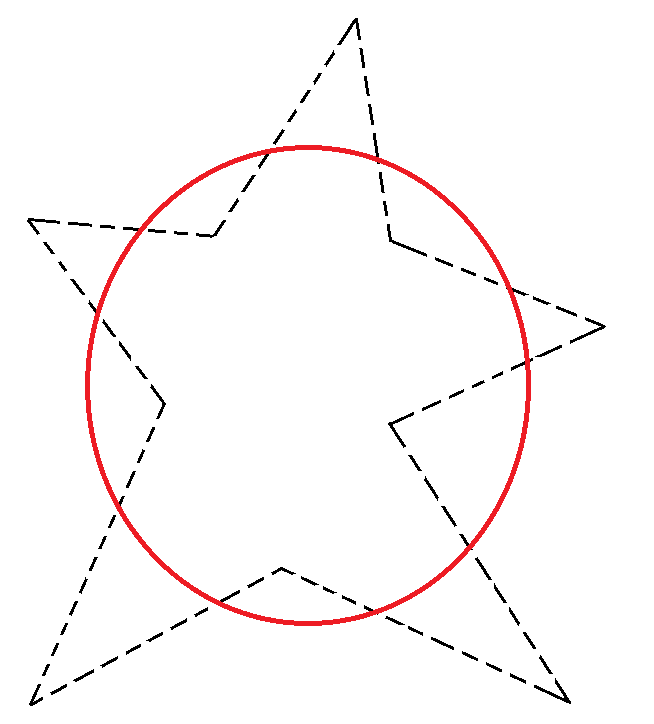
\includegraphics[width=0.5\textwidth]{conculsion4.png}
\captionsetup{font={scriptsize}}
\caption*{Penalization \& Subsidization}
\end{minipage}
\end{figure}
\vspace{-15mm}
\end{frame}


\begin{frame}{Instrument 2: Simultaneous P\&S, {\footnotesize 2018, OR}}{Instrument of Penalization (Least Core)}
\vspace{3mm}
{\footnotesize $\mathrm{Core}(N,\pi) = \bigg\{ \alpha:~ \alpha(N)=\pi(N), ~\alpha(S) \leq \pi(S), ~\forall S \in \mathbb{S} \setminus \{N\},~\alpha \in \R^n   \bigg\}$.}
\begin{shaded}
\centering \textcolor{red}{\bf Relax Coalition Stability constraints}: $\alpha(S) \leq \pi(S)$
\end{shaded}
\begin{itemize}
\item \textcolor{blue}{Minimum Penalty} to stabilize the grand coalition:
\small
\begin{equation*}
z^* = \min \big\{ z:\alpha(N)= \pi(N),~\alpha(S) \leq \pi(S)+z, ~\forall S \in \mathbb{S} \setminus \{N\} \big\}.
\end{equation*}
\end{itemize}
\pause
\vspace{-7mm}
\begin{shaded}
\centering
\small
Minimum Penalty needed for MSG Example:\\
\vspace{2mm}
\textcolor{red}{$z^* = 0.5$}
\end{shaded}
\end{frame}



\begin{frame}{Instrument 2: Simultaneous P\&S, {\footnotesize 2018, OR}}{Penalty-Subsidy Pair}
\vspace{3mm}
{\footnotesize $\mathrm{Core}(N,\pi) = \bigg\{ \alpha:~ \alpha(N)=\pi(N), ~\alpha(S) \leq \pi(S), ~\forall S \in \mathbb{S} \setminus \{N\},~\alpha \in \R^n   \bigg\}$.}
\begin{shaded}
\centering \textcolor{red}{\bf \small Relax Coalition Stability and Budget Balance constraints}
\end{shaded}
\begin{itemize}
\item \textcolor{blue}{Penalty-Subsidy Pair} to stabilize the grand coalition:
\small
\begin{equation*}
\omega(z) = \min_{\alpha} \bigg\{ \pi(N) - \alpha(N):~\alpha(S) \leq \pi(S)+z,~\forall S \in \mathbb{S} \setminus \{N\} \bigg\}
\end{equation*}
\end{itemize}
\pause
\vspace{-7mm}
\begin{shaded}
\centering
\small
Penalty-Subsidy Pair for MSG Example:\\
\vspace{2mm}
\textcolor{red}{E.g., combination of penalty 0.1667 and subsidy 0.5}
\end{shaded}
\end{frame}


%\begin{frame}{Instrument 2: Simultaneous P\&S, {\footnotesize 2018, OR}}{Research Questions}
%\justifying
%\begin{shaded}
%\small
%Compute a \textcolor{red}{\bf combination of subsidy and penalty} such that
%\begin{itemize}
%\item  the cost assigned to each coalition \textcolor{red}{\bf does not exceed the total cost incurred plus the penalty} if they deviate;
%\item the total assigned cost \textcolor{red}{\bf plus the subsidy is equal to} the total cost incurred by grand cooperation.
%\end{itemize}
%\end{shaded}
%\end{frame}

\begin{frame}{Instrument 2: Simultaneous P\&S, {\footnotesize 2018, OR}}{Research Questions}
\justifying
\textcolor{red}{How to use penalty and subsidy simultaneously to stabilize the grand cooperation? What's the trade-off?}\\
\begin{figure}
	%\caption{Illustration of the construction of the PSF $\omega(z)$ by the IPC algorithm.}
	\centering{
		\scalebox{0.3}{
			\adjustbox{trim={.08\width} {.01\height} {0.08\width} {.05\height},clip}
			{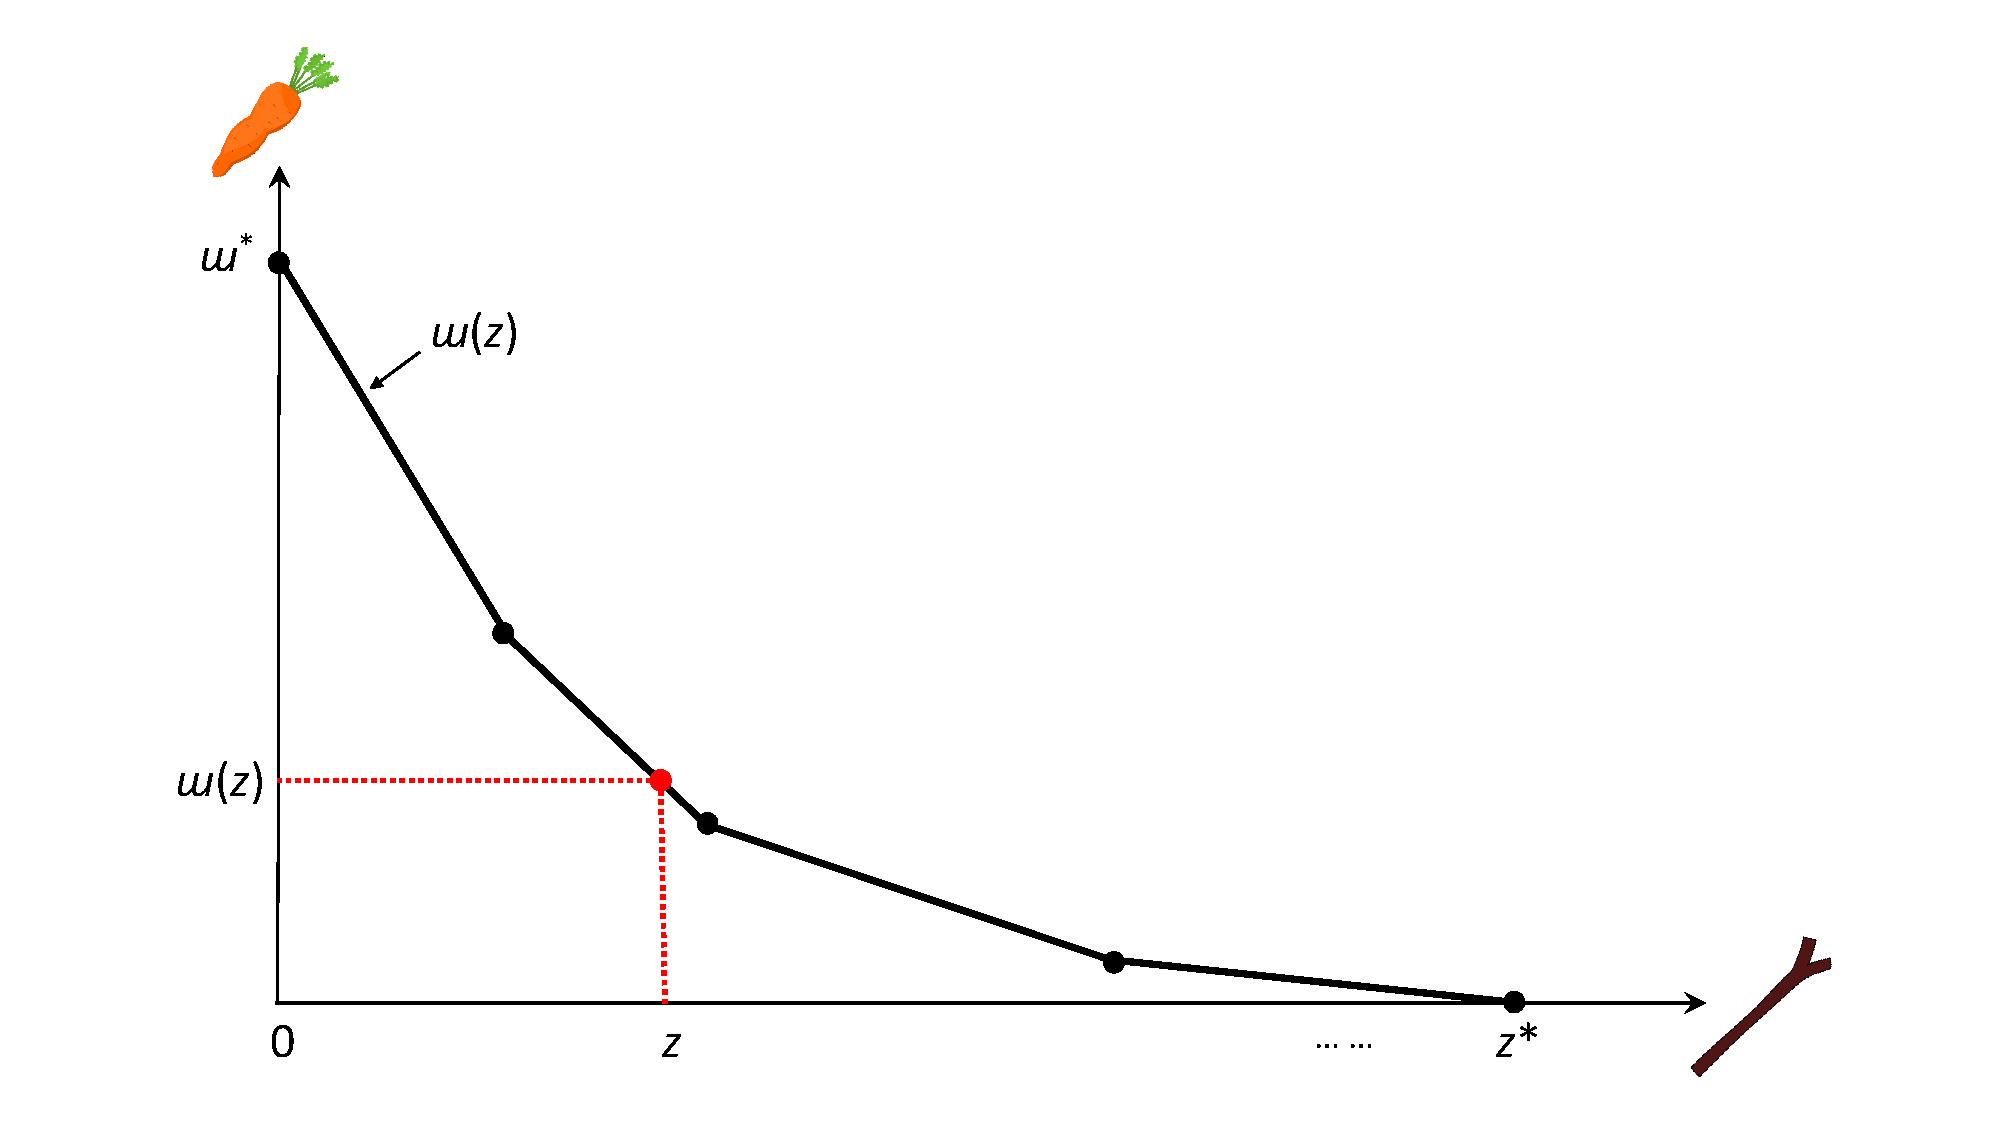
\includegraphics{figure-carrot-stick.pdf}}
		}
	}
\end{figure}
\end{frame}



\begin{frame}{Instrument 2: Simultaneous P\&S, {\footnotesize 2018, OR}}{Penalty Subsidy Function $\omega(z)$ -- Properties}
\small
\begin{theorem}
\rm
	\begin{itemize}
	\justifying
%		\item	$\omega(0) = \omega^*$, $\omega(z^*)=0$, and $0 < \omega(z) < \omega^*$ for any $z \in \big(0,z^*\big)$.
		\item $\omega(z)$ is \textcolor{red}{decreasing}, \textcolor{red}{piecewise linear}, and \textcolor{red}{convex} in $z \in\big[ 0,z^* \big]$.
\item For each segment of $\omega(z)$, the \textcolor{red}{slope $\omega'(z) \in \big[ -n, -\frac{n}{n-1}\big]$}.
	\end{itemize}
\end{theorem}
\begin{shaded}
\vspace{-2mm}
\begin{itemize}
\justifying
	\item Decreasing of $\omega(z)$: trade-off between penalty and subsidy;
	\item Convexity of $\omega(z)$: diminishing effect on increasing the penalty to reduce the minimum subsidy desired.
	%\item $\omega'(z) \in \big[ -n, -\frac{n}{n-1}\big]$: challenges in the construction of $\omega(z)$.
\end{itemize}
\vspace{-2mm}
\end{shaded}
\end{frame}


%\begin{frame}{Instrument 2: Simultaneous P\&S, {\footnotesize 2018, OR}}{Intersection Points Computation (IPC) Algorithm}
%\setbeamersize{description width=0.1cm}
%\small
%\justifying
%	\begin{description}
%		\item[Step 1.] Set $P^* = \big\{0,z^*\big\}$ and $\mathbb{P} = \big\{ \big[0,z^*\big]\big\}$.
%		\vspace{2mm}
%		\item[Step 2.] Until $\mathbb{P}$ is empty, update $P^*$ and $\mathbb{P}$ as follows:
%		\begin{itemize}
%		\justifying
%		\small
%			\item $P^*$: $0=z_0<\cdots<z_q=z^*$.
%			\vspace{2mm}
%			\item Remove any \textcolor{red}{interval $\big[z_{k-1},z_k\big]$} from $\mathbb{P}$.
%			\vspace{2mm}
%			\item Construct \textcolor{red}{linear functions $R_{k-1}(z)$ and $L_{k}(z)$}.
%			\vspace{2mm}
%%			\begin{itemize}
%%				\item $R_{k-1}(z)$ passes $\big(z_{k-1},\omega(z_{k-1})\big)$ with a slope equal to a right weak derivative of $\omega(z)$ at $z_{k-1}$;
%%				\item $L_{k}(z)$ passes $\big(z_{k},\omega(z_{k})\big)$ with a slope equal to a left weak derivative of $\omega(z)$ at $z_{k}$.
%%			\end{itemize}
%			\item If $R_{k-1}(z)$ and $L_{k}(z)$ \textcolor{red}{intersect} at $z' \in \big(z_{k-1},z_k\big)$, add $z'$ to $P^*$, add $\big[z_l,z'\big]$, $\big[z',z_{r}\big]$ to $\mathbb{P}$.
%		\end{itemize}
%		\vspace{2mm}
%		\item[Step 3.] %Return a piecewise linear function that
%		 \textcolor{red}{Connect $\big(z,\omega(z)\big)$} for $z\in P^*$.
%	\end{description}
%%\end{algorithm}
%\end{frame}

\begin{frame}{Instrument 2: Simultaneous P\&S, {\footnotesize 2018, OR}}{Intersection Points Computation Algorithm: Illustrations on Scheduling Game}
\small
\vspace{-7mm}
\begin{figure}[t]
	\label{figure:IPCExample}
	\centering{
		\scalebox{0.68}{
			\adjustbox{trim={.14\width} {.49\height} {0.05\width} {.25\height},clip}{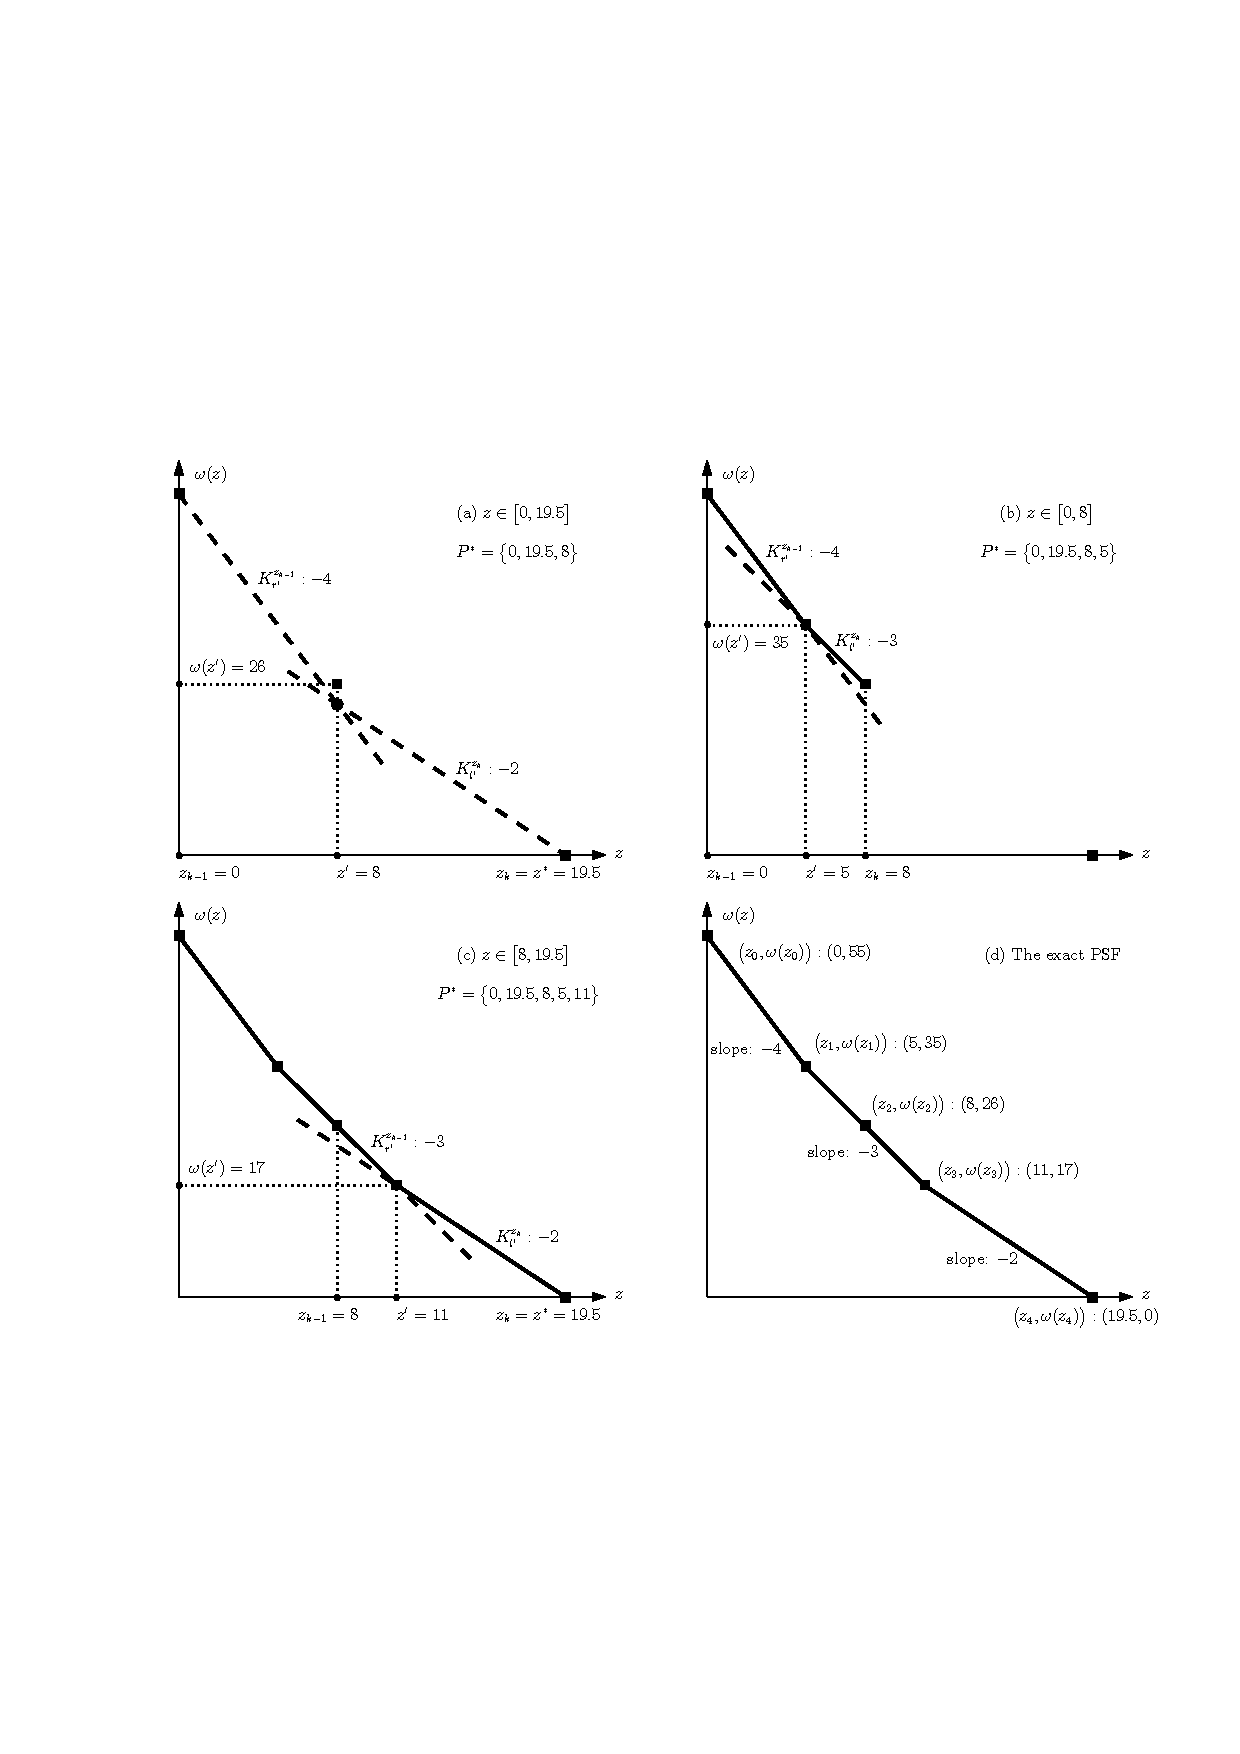
\includegraphics{figure2-170616g.pdf}}
		}
	}
	\vspace{-8mm}
\end{figure}
\end{frame}

\begin{frame}{Instrument 2: Simultaneous P\&S, {\footnotesize 2018, OR}}{Intersection Points Computation Algorithm: Illustrations on Scheduling Game}
\small
\vspace{-7mm}
\begin{figure}[t]
	\label{figure:IPCExample1}
	\centering{
		\scalebox{0.68}{
			\adjustbox{trim={.14\width} {.24\height} {0.05\width} {.51\height},clip}{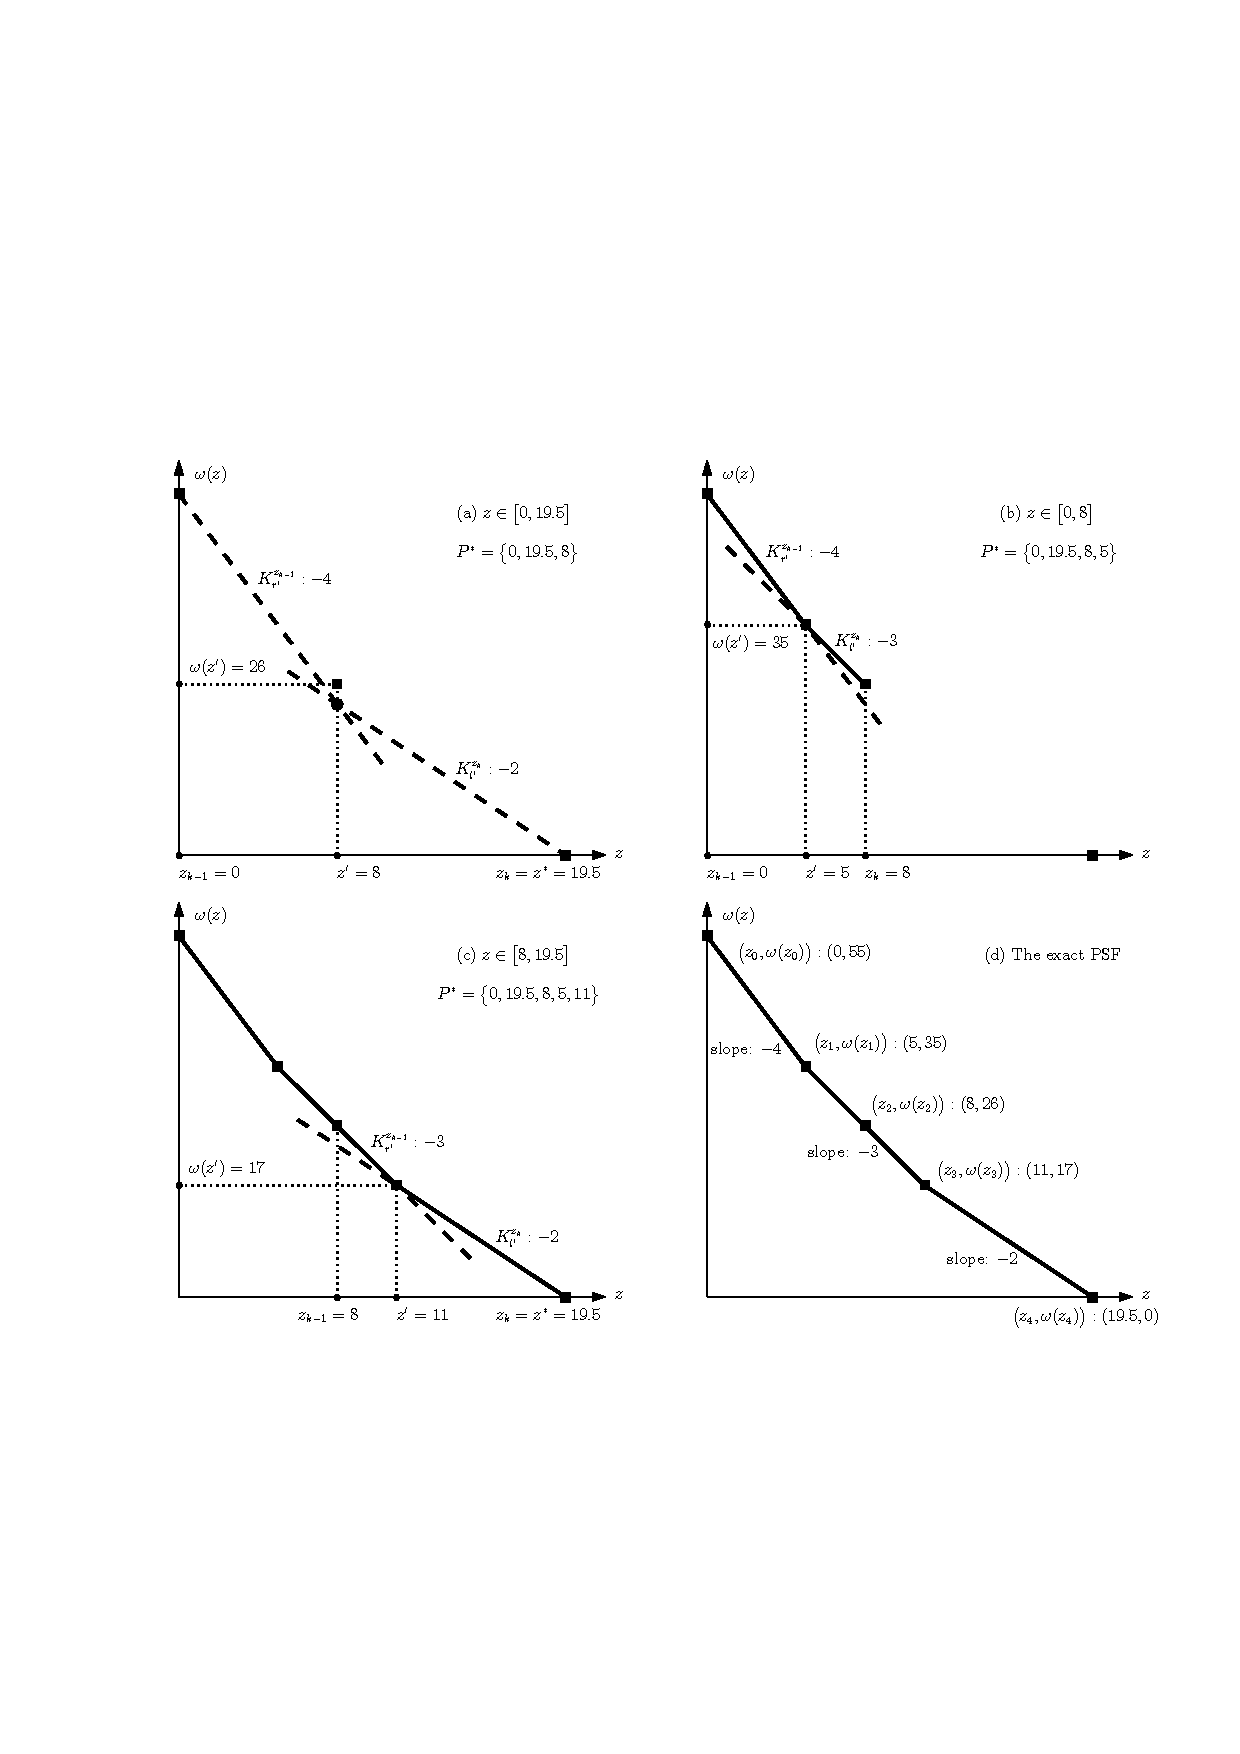
\includegraphics{figure2-170616g.pdf}}
		}
	}
	\vspace{-8mm}
\end{figure}
\end{frame}

\begin{frame}{Instrument 2: Simultaneous P\&S, {\footnotesize 2018, OR}}{Efficiency of the IPC Algorithm}
\vspace{-6pt}
\small
\begin{theorem}
\rm
\justifying
	If function $\omega(z)$ has \textcolor{red}{$\hat{q}\geq 2$} linear segments, then the IPC algorithm will terminate after at most \textcolor{red}{$4\hat{q}-1$} iterations.
\end{theorem}
\vspace{-11pt}
\begin{figure}
	%\caption{Illustration of the construction of the PSF $\omega(z)$ by the IPC algorithm.}
	\centering{
		\scalebox{0.40}{
			\adjustbox{trim={.1\width} {.19\height} {0.01\width} {.19\height},clip}
			{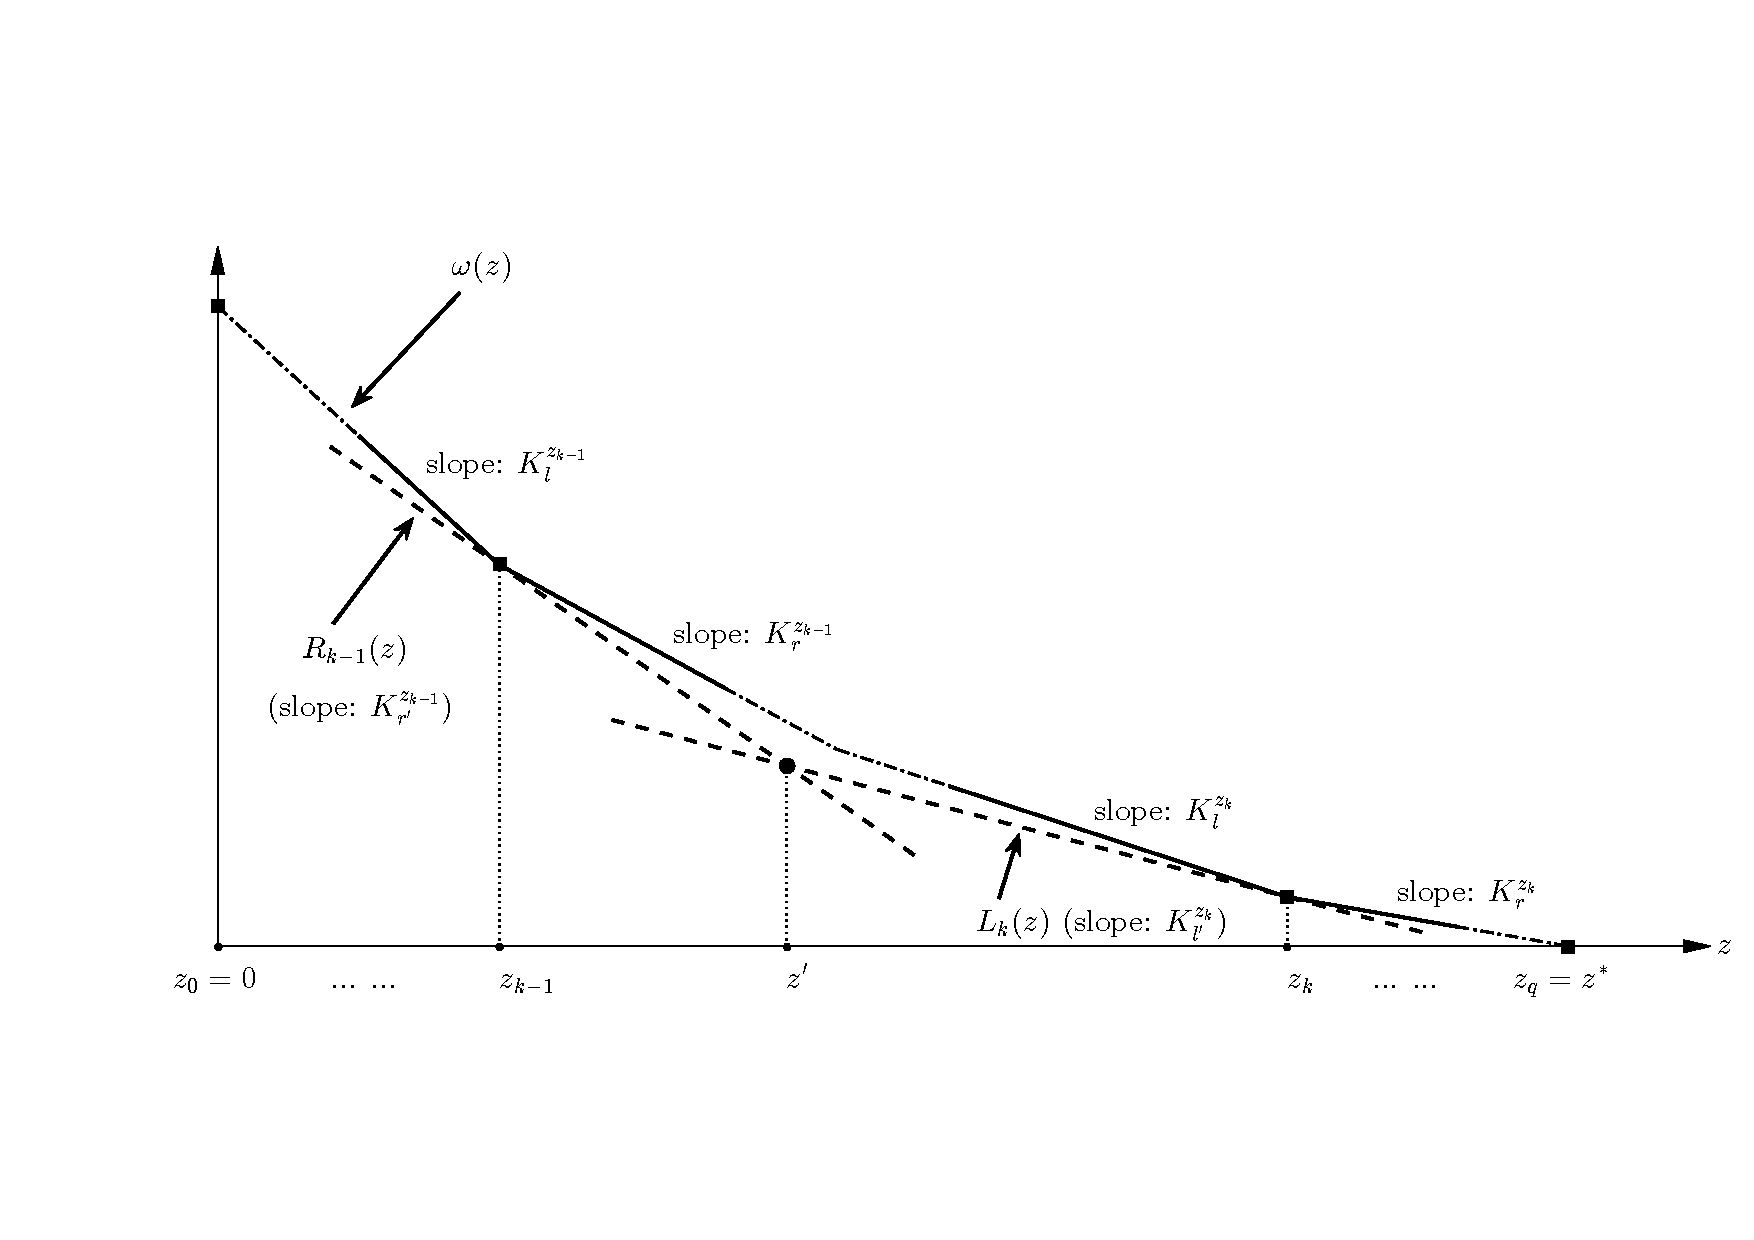
\includegraphics{figure1-170616g.pdf}}
		}
	}
\end{figure}
\vspace{-20pt}
\end{frame}

\begin{frame}{Instrument 2: Simultaneous P\&S, {\footnotesize 2018, OR}}{Heuristic to Construct $\omega(z)$: $\epsilon$-Approximation}
\small
%\setbeamersize{description width=1cm}
%\begin{description}
%\justifying
%	\item[Step 1.] Evenly divide $\big[0,z^*\big]$ into $\lceil 2v/\epsilon\rceil$ sub-intervals denoted by $\big[z_0,z_1\big)$, $\ldots$, $\big[z_{\lceil 2v/\epsilon\rceil-1},z_{\lceil 2v/\epsilon\rceil}]$;
%	\item[Step 2.] For each $0\leq i\leq \lceil 2v/\epsilon\rceil$, compute  $\omega(z_i)$;
%	\item[Step 3.] Obtain an upper bound $U_{\epsilon}(z)$ for $\omega(z)$ by joining points in $\big\{\big(z_0,\omega(z_0)\big),\ldots,\big(z_{\lceil 2v/\epsilon\rceil},\omega(z_{\lceil 2v/\epsilon\rceil})\big) \big\}$.
%\end{description}
\setbeamersize{description width=1cm}
\begin{description}
\justifying
	\item[Step 1.] Evenly divide $\big[0,z^*\big]$ into $\lceil 2v/\epsilon\rceil$ sub-intervals;
	\item[Step 2.] For each sub-interval, compute $\big(z_i,\omega(z_i)\big)$;
	\item[Step 3.] Obtain upper bound $U_{\epsilon}(z)$ for $\omega(z)$ by linking these points.
\end{description}
\vspace{-1mm}
\begin{theorem}\label{thm:epsilonapproximation}
\justifying
\rm
\small
$E_c \leq \big(\epsilon/2\big) \big(z^* \big)^2 \leq \epsilon$ {$\int_0^{z^*}\omega(z) \,\mathrm{d}z$} and $E_{\max}\leq$ {$\big($}$\epsilon$ {$z^*\big)/2$}, $\big(\epsilon>0\big)$.
\end{theorem}
\vspace{4mm}
\textcolor{red}{Cumulative error}: $E_c = \int_0^{z^*} \big| U_{\epsilon}(z)-\omega(z) \big| \,\mathrm{d} z$,\\
\textcolor{red}{Maximum error}: $E_{\max}=\max_{z\in \big[0,z^*\big]}\big\{|U_{\epsilon}(z)-\omega(z)|\big\}$.
\end{frame}



\begin{frame}{Instrument 2: Simultaneous P\&S, {\footnotesize 2018, OR}}{How to compute $\omega(z)$ for given penalty $z$?}
%(Required by the IPC and the $\epsilon$-approximation algorithms.)
\vspace{-30pt}
\small
\begin{eqnarray*}
	\omega(z) = &&\min_{\alpha}\bigg\{ \pi(N) - \alpha(N):\\
	&& \alpha(S) \leq \pi(S)+z \mbox{ for all } S \in \mathbb{S} \setminus \{N\},~\alpha \in \R^n \bigg\}.
\end{eqnarray*}
Define:
\vspace{-10pt}
\begin{eqnarray*}
\tau(z) = && \max_{\alpha} \bigg\{ \alpha(N): \\
&& \alpha(S) \leq \pi(S)+z \mbox{ for all } S \in \mathbb{S} \setminus \{N\},~ \alpha \in \R^n \bigg\}.
\end{eqnarray*}
\textcolor{red}{We obtain that $\omega(z) = c(N)-\tau(z)$.}
\end{frame}



\begin{frame}{Instrument 2: Simultaneous P\&S, {\footnotesize 2018, OR}}{Cutting-Plane (CP) Approach to Computing $\omega(z)$ for Given $z$}
\small
%Recall: $\omega(z) = c(N)-\pi(z)$, where
%$$\pi(z) = \max_{\alpha\in \R^n} \big\{ \alpha(N): \alpha(s) \leq c(s)+z \textcolor{red}{\mbox{ for all } s \in S \setminus \{N\}}\}.$$
%\pause
\setbeamersize{description width=0.1cm}
\begin{description}
\justifying
\item[Step 1.] $\mathbb{S}'\subseteq \mathbb{S}\setminus \{N\}$ indicates a \textcolor{red}{restricted coalition set}.
\item[Step 2.] Find an optimal $\bar{\alpha}(\ \cdot \ ,z)$ to \textcolor{red}{a relaxed LP} of $\tau(z)$:
\begin{equation*}
\max_{\alpha\in \R^n} \big\{ \alpha(N,z): \alpha(S,z) \leq \pi(S)+z, \mbox{ for all } S \in \mathbb{S}'\big\}.
\end{equation*}
\vspace{-11pt}
\item[Step 3.]
Find an optimal $S^*$ to the \textcolor{red}{separation problem}:
\begin{equation*}
\delta = \min \big\{ \pi(S)+z-\bar{\alpha}(S,z): \forall S \in \mathbb{S} \setminus \{N\}\big\}.
\end{equation*}
\item[Step 4.]
If \textcolor{red}{$\delta<0$}, then add $S^*$ to $\mathbb{S}'$, and go to step 2; otherwise, return \textcolor{red}{$\omega(z)=\pi(N)-\bar{\alpha}(N,z)$}. %; and (ii) a pair of weak derivatives $\big( K_{l'}^{\bar{\alpha}z},K_{r'}^{\bar{\alpha}z}\big)$ computed by solving (\ref{eqn:weakderivatives}) with $S^{\alpha z}$ replaced by $S'$ in the definition of $\Pi^{\alpha z}$.
\end{description}
\begin{shaded}
\centering
Generate \textcolor{red}{a lower bound} when serving as a heuristic
\end{shaded}
\end{frame}



\begin{frame}{Instrument 2: Simultaneous P\&S, {\footnotesize 2018, OR}}{Linear Programming (LP) Approach to Computing $\omega(z)$ for a Given $z$}
\small
Inspired by Caprara \& Letchford (2010) for $\tau(0)$, define:
{\small
\begin{eqnarray*}
Q^{x\mu y} = \big\{(x,\mu,y):Ax \geq By+D\mu, y = y^s\mbox{~for some $s \in S \setminus \{N\}$},\\
 \mu=1,~x \in \Z^{ t},~y \in \big\{0,1\big\}^{n}\big\},\\
 C^{x\mu} = \mathrm{proj}_{x\mu} \big( \big\{ (x,\mu,y) \in \R^{t+1+n}:  y = \mathbf{1} \big\} \cap \mathrm{cone~} Q^{x\mu y} \big).
\end{eqnarray*}
}
\vspace{-6mm}
\begin{theorem}
\centering
	$\tau(z)=\min \big\{ cx + z\mu: (x,\mu) \in C^{x\mu} \big\}$.
\end{theorem}
\begin{shaded}
\centering
Generate \textcolor{red}{an upper bound} when serving as a heuristic
\end{shaded}
\end{frame}


\begin{frame}{Instrument 2: Simultaneous P\&S, {\footnotesize 2018, OR}}{Applications}

{\small
Parallel Machine Scheduling Games:
\begin{itemize}
\small
	\item Players $N = \{1,\ldots,n\}$; Machines $M = \{1,\ldots,m\}$.
	\item Each coalition $S$ minimizes the total (weighted) completion time of jobs of players in $S$. % on machines in $M$.
\end{itemize}
\vspace{3pt}
\textcolor{blue}{Results on computing $\omega(z)$ for given $z$:}
\begin{table}[H]
\small
	\vspace{-5pt}
	\centering
	\tabcolsep=3pt
\footnotesize
	\renewcommand\arraystretch{1.35}
	%\caption{\label{table:PMSClass} The demonstration results on the four types of PMS games}
%	\vglue5pt
	\begin{tabular}[!h]{c c c c c}
		\hline
		\multicolumn{1}{c}{} &\multicolumn{1}{c}{Machines} &\multicolumn{1}{c}{Jobs}	&\multicolumn{1}{c}{CP Approach}	&\multicolumn{1}{c}{LP Approach}\\
		\hline
		IPU		&\textcolor{black}{Identical}		&\textcolor{black}{Unweighted} 	&\textcolor{red}{P-time}	&\textcolor{red}{P-time}\\

		UPU		&\textcolor{black}{Unrelated}	&\textcolor{black}{Unweighted}	&--	&\textcolor{red}{P-time}\\

		IPW		&\textcolor{black}{Identical}		&\textcolor{black}{Weighted}	&\textcolor{red}{Pseudo P-time} (fixed $m$)	&--		\\

		UPW		&\textcolor{black}{Unrelated}	&\textcolor{black}{Weighted}	&\textcolor{red}{Lower Bound}	&\textcolor{red}{Upper Bound}\\
		\hline
	\end{tabular}
%	\vspace{-2mm}
\end{table}
}
\end{frame}


\begin{frame}{Instrument 2: Simultaneous P\&S, {\footnotesize 2018, OR}}{Conclusions}
\centering
\begin{itemize}
\normalsize
\justifying
\item[$\star$] \textcolor{purple}{Cooperative Game Theory}:
\begin{itemize}
\small
\vspace{2mm}
\item[$-$] {\color{blue}{New Instrument}} for Stabilization via Simultaneous P\&S.
\vspace{2mm}
\end{itemize}
\item[$\star$] \textcolor{purple}{Models, Solution Methods}:
\begin{itemize}
\small
\vspace{2mm}
\item[$-$] Characterize {\color{blue}{properties}} of the penalty-subsidy function $\omega(z)$, revealing the trade-off;
\vspace{2mm}
\item[$-$] Develop {\color{blue}{two algorithms}} to construct function $\omega(z)$;
\vspace{2mm}
\item[$-$] Develop {\color{blue}{two solution approaches}} to computing the values of $\omega(z)$ for any given $z$.
\vspace{2mm}
\end{itemize}
\item[$\star$] \textcolor{purple}{Applications}:
\begin{itemize}
\small
\vspace{2mm}
	\item[$-$] Implementations on several machine scheduling games.
\end{itemize}
\end{itemize}
\end{frame}



\subsection{Instrument of Cost Adjustment}
\begin{frame}
\centering
\normalsize
\textcolor{olive}{\bf {\LARGE 3.} \bf {\LARGE I}NSTRUMENT OF {\bf {\LARGE C}}OST {\bf {\LARGE A}}DJUSTMENT}
\vspace{5mm}
\begin{figure}[H]
\centering
\begin{minipage}[t]{0.32\textwidth}
\centering

\includegraphics[width=0.5\textwidth]{conculsion1.png}
\captionsetup{font={scriptsize}}
\caption*{Unbalanced Game}
\end{minipage}
\begin{minipage}[t]{0.32\textwidth}
\centering
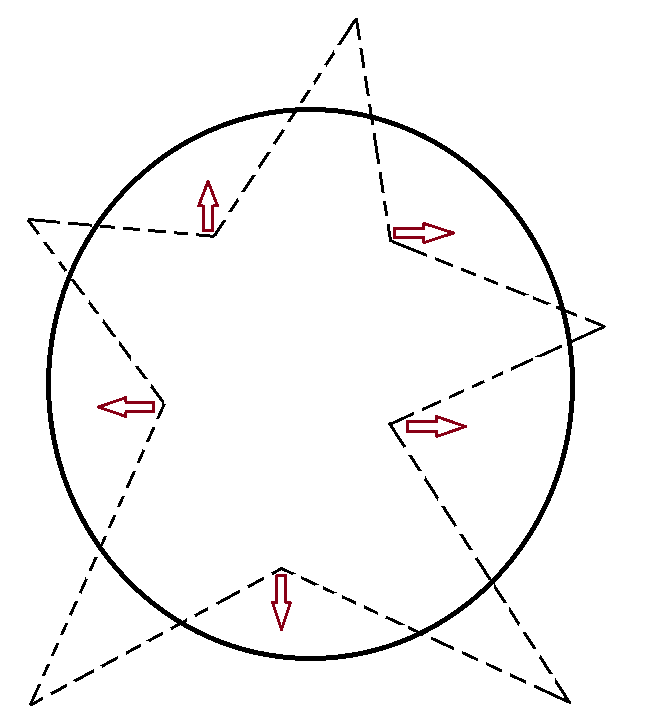
\includegraphics[width=0.5\textwidth]{conculsion5.png}
\captionsetup{font={scriptsize}}
\caption*{Cost Adjustment}
\end{minipage}
\end{figure}
\vspace{-15mm}
\end{frame}


\begin{frame}{Instrument 3: Cost Adjustment, {\footnotesize 2019, Under Review}}{Ex-post Actions}
\vspace{-5mm}
\begin{shaded}
\small
\centering
\textcolor{red}{\bf Ex-post actions} on $\mathrm{Core}(N,\pi)$
\end{shaded}
\vspace{-5mm}
\begin{small}
\vspace{-5mm}
\begin{eqnarray*}
\mathrm{Core}(N,\pi) = \bigg\{ \alpha:~ \alpha(N)=\pi(N),  ~\alpha(S) \leq \pi(S), ~\forall S \in \mathbb{S} \setminus \{N\}  \bigg\}
\end{eqnarray*}
\end{small}
\vspace{-5mm}
\begin{itemize}
\small
\item Subsidization: \textcolor{red}{$\alpha(N)=\pi(N)-\theta$}, \textbf{$\epsilon-$core};
\item Penalization: \textcolor{red}{$\alpha(S) \leq \pi(S)+z$}, \textbf{least core};
\item Simult. S \& P: \textcolor{red}{$\alpha(N)=\pi(N)-\theta$ and $\alpha(S) \leq \pi(S)+z$}, \textbf{PSF}.
\end{itemize}
\end{frame}



\begin{frame}{Instrument 3: Cost Adjustment, {\footnotesize 2019, Under Review}}{Illustrative Example: Braess's Paradox}
\vspace{-5mm}
\begin{figure}[H]
\centering
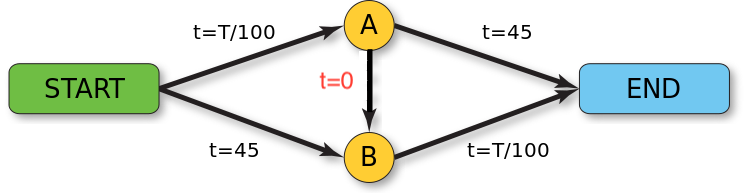
\includegraphics[width=1\textwidth]{braess.png}
\end{figure}
\centering
\vspace{-6mm}
4000 cars in total
\vspace{4mm}
\begin{columns}
\begin{column}{5.5cm}
\small
\centering
$t = 0$\\
\vspace{2mm}
$START \rightarrow A \rightarrow B \rightarrow END$\\
\vspace{2mm}
$4000/100  + 4000/100 = 80 min$
\end{column}
\begin{column}{5.5cm}
\small
\centering
\pause
\textcolor{red}{$t = \infty$}\\
\vspace{2mm}
$START \rightarrow A  \rightarrow END$\\
\vspace{2mm}
$START  \rightarrow B \rightarrow END$\\
\vspace{2mm}
$A=B=2000$\\
\vspace{2mm}
$2000/100+45=65min$
\end{column}
\vspace{-5mm}
\end{columns}
\vspace{-5mm}
\end{frame}



\begin{frame}{Instrument 3: Cost Adjustment, {\footnotesize 2019, Under Review}}{Ex-ante Action}
\justifying
\small
\begin{eqnarray*}
\mathrm{Core}(N,\pi) = \bigg\{ \alpha:~ \alpha(N)=\pi(N;c), ~\alpha(S) \leq \pi(S;c), ~\forall S \in \mathbb{S}    \bigg\}.
\end{eqnarray*}
\begin{equation*}
\pi(S;c) = \min_{x} \{ cx: Ax \geq By^S + E, ~x \in \Z^{q} \}.
\end{equation*}
\begin{shaded}
\textcolor{red}{\bf Ex-ante Action}\\
~\\
~~~~~~~~~~~~~~Cost Adjustment: \textcolor{cyan}{$ c \rightarrow d$ and $\pi(S;c) \rightarrow \pi(S;d)$}
\end{shaded}
\end{frame}



%\begin{frame}{An Illustrative Example on UFL Game}
%\small
%\begin{columns}
%\begin{column}{5.5cm}
%\vspace{-10mm}
%\begin{figure}[H]
%\centering
%\includegraphics[width=1.05\textwidth]{UFL1.pdf}
%\end{figure}
%\end{column}
%\begin{column}{5.5cm}
%\vspace{-5mm}
%\footnotesize
%\begin{shaded}
%Social Optimum $\pi(N)$:
%\begin{equation*}
%10+10+1+1+1=23
%\end{equation*}
%\vspace{-5mm}
%\end{shaded}
%\vspace{-10mm}
%\begin{shaded}
%Optimal Cost Allocation Problem:
%\begin{eqnarray*}
%\begin{aligned}
%\max ~\alpha_1 + &\alpha_2 + \alpha_3\\
%s.t.~~ \alpha_1 \leq 11,~\alpha_2& \leq 11,~\alpha_3 \leq 11,\\
%\alpha_1 + \alpha_2& \leq 12,\\
%~\alpha_1+\alpha_3 \leq 12,&~\alpha_2+\alpha_3 \leq 12,\\
%\alpha_1 + \alpha_2 + &\alpha_3 \leq 23.
%\end{aligned}
%\end{eqnarray*}
%\vspace{-5mm}
%\end{shaded}
%\vspace{-10mm}
%\begin{shaded}
%Optimal Cost Allocation:
%\begin{equation*}
%6+6+6=18 < 23 \mbox{~(not stable)}
%\end{equation*}
%\vspace{-5mm}
%\end{shaded}
%\end{column}
%\end{columns}
%\end{frame}
%
%\begin{frame}{An Illustrative Example on UFL Game}
%\small
%\begin{columns}
%\begin{column}{5cm}
%\vspace{-15mm}
%\begin{figure}[H]
%\centering
%%\caption{\label{figure:example}An example of UFL game}
%\centering
%\includegraphics[width=1.05\textwidth]{UFL2.pdf}
%\end{figure}
%\end{column}
%\begin{column}{6cm}
%\footnotesize
%\vspace{-10mm}
%\begin{shaded}
%Optimal Cost Allocation Problem:
%\begin{eqnarray*}
%\begin{aligned}
%\max ~\alpha_1 + &\alpha_2 + \alpha_3\\
%s.t.~~ \alpha_1 \leq 11,~\alpha_2& \leq 11,~\alpha_3 \leq 11,\\
%\alpha_1 + \alpha_2& \leq \textcolor{red}{22},\\
%~\alpha_1+\alpha_3 \leq 12,&~\alpha_2+\alpha_3 \leq 12,\\
%\alpha_1 + \alpha_2 + &\alpha_3 \leq 23.
%\end{aligned}
%\end{eqnarray*}
%\vspace{-5mm}
%\end{shaded}
%\vspace{-10mm}
%\begin{shaded}
%\centering
%($c_{22}=1 \rightarrow 11$): \\
%Optimal Cost Allocation
%$$
%11+11+1=23 \mbox{~(stabilized)}
%$$
%\vspace{-6mm}
%\end{shaded}
%\vspace{-10mm}
%\begin{shaded}
%\centering
%Social Optimum: unchanged\\
%\vspace{1mm}
%Optimal Solution: unchanged
%\end{shaded}
%\vspace{-10mm}
%\end{column}
%\end{columns}
%\end{frame}



%
%
%\begin{frame}{Properties of an IM Game}
%\vspace{-5mm}
%\begin{shaded}
%\centering
%\small
%IM Game $(V,C)$: $\pi(S) = \min_{x} \{ cx: Ax \geq By^S + E, ~x \in \Z^{t} \}$
%\end{shaded}
%\vspace{-8mm}
%\begin{table}
%\centering
%\scriptsize
%\tabcolsep=0pt
%\renewcommand\arraystretch{1.9}
%\begin{tabular}[!h]{c c c}
%\hline
%\multicolumn{1}{c}{Parameters} &\multicolumn{1}{c}{Properties}	&\multicolumn{1}{c}{Explanations}\\
%\hline
%\multicolumn{1}{c}{$B \geq \textbf{0}$} &\multicolumn{1}{c}{Monotonicity}	&\multicolumn{1}{c}{$C(S \cup \{k\}) \geq \pi(S)$ for all $S \in \mathbb{S}, ~k\in V$:$~S \cup \{k\} \in \mathbb{S}$;}\\
%\multicolumn{1}{c}{$B = \textbf{0}$} &\multicolumn{1}{c}{Coalitional-Independence}	&\multicolumn{1}{c}{$\pi(S)$ for all $S \in \mathbb{S}$ are identical;}\\
%\multirow{2}{*}{$E \geq \textbf{0}$} &\multirow{2}{*}{Subadditivity}	&\multicolumn{1}{l}{$C(S_1 \cup S_2) \leq C(S_1)+C(S_2)$ for all $S_1, S_2 \in \mathbb{S}:$}\\
%&	&\multicolumn{1}{r}{$S_1 \cup S_2 \in \mathbb{S},~ S_1 \cap S_2 = \emptyset$;}\\
%\hdashline
%\multicolumn{1}{c}{$E = \textbf{0}$} &\multicolumn{1}{c}{Homogeneity (Assignability)}	&\multicolumn{1}{c}{$\alpha^*(V) \leq \min_x \big\{ cx:Ax \geq B\textbf{1} + E, ~x \in \R_{+}^{q} \big\}$;}\\
%\multicolumn{1}{c}{$A =$\textbf{\uppercase\expandafter{\romannumeral2}},} &\multirow{2}{*}{Complete Assignability}	&\multirow{2}{*}{$\alpha^*(V)= \min_x \big\{ cx:Ax \geq B\textbf{1} + E, ~x \in \R_{+}^{q} \big\}$.}\\
%\multicolumn{1}{c}{$B = \textbf{I}$, $E = \textbf{0}$} &	&\\
%\hline
%\end{tabular}
%\end{table}
%\vspace{-5mm}
%\begin{tablenotes}
%\tiny
%\centering
% \item[1] $\alpha^*(V)=\max_{\alpha}\big\{ \alpha(V):\alpha(S) \leq \pi(S), ~\forall S \in \mathbb{S} \big\}$;
%        ~$\textbf{0}$, $\textbf{1}$, \textbf{\uppercase\expandafter{\romannumeral2}}, $\textbf{I}$: all-zeros, all-ones, binary, identity matrices
%      \end{tablenotes}
%\end{frame}


\begin{frame}{Instrument 3: Cost Adjustment, {\footnotesize 2019, Under Review}}{Stabilization via Cost Adjustment}
\begin{definition}\label{definition:inverse}
\small
\justifying
Grand Coalition Stabilization Problem (GCSP) via Cost Adjustment (CA):\\
\centering \textcolor{blue}{\bf $c \rightarrow d$}, such that \textcolor{red}{\bf BCC}
\begin{itemize}
\item \textcolor{red}{Balancedness:} the updated IM game $\big(N,\pi(\~\cdot\~;d)\big)$ is balanced;
\item \textcolor{red}{Cooperation Scheme:} an initial $x^0$ is optimal to $\pi(N;d)$;
\item \textcolor{red}{Cost Sharing:} total cost $\pi(N;d)$ to share is within $\big[l,u\big]$.
\end{itemize}
\vspace{-3mm}
\end{definition}
\begin{shaded}
\small
{\bf Ex-post actions on $\mathrm{Core}(N,\pi)$
~V.S.~
Ex-ante action on $\pi(\~\cdot\~,c)$}
\end{shaded}
\end{frame}

\begin{frame}{Instrument 3: Cost Adjustment, {\footnotesize 2019, Under Review}}{Constrained Inverse Optimization}
\vspace{-3mm}
\begin{shaded}
\centering
Constrained Inverse Optimization Problem (CIOP)
\end{shaded}
\vspace{-5mm}
\footnotesize
\begin{eqnarray*}
\min \bigg\{ f(\delta): \mathrm{Core}\big|\big(N,\pi(\~\cdot\~;d)\big)\big| \geq 1, ~dx^0 = \pi(N;d),~l \leq \pi(N;d) \leq u,~
d \in \R^{q}\bigg\}.
\end{eqnarray*}
\begin{itemize}
\small
\item Only Optimality: \textcolor{red}{Inverse Optimal Solution} Problem;
\item Only Consistency: \textcolor{red}{Inverse Optimal Value} Problem;
\item Only Balancedness: \textcolor{red}{Optimal Cost Allocation} Problem.
\end{itemize}
\end{frame}




\begin{frame}{Instrument 3: Cost Adjustment, {\footnotesize 2019, Under Review}}{$\mathcal{NP}$-hardness and Feasibility}
\begin{theorem}
\justifying
\small
\centering
\textbf{\rm Solving the CIOP is in general $\mathcal{NP}$-hard.}
\end{theorem}
\begin{theorem}\label{theorem:SAndN}
\justifying
\small
\centering
\textbf{\rm Feasibility -- Sufficient and Necessary Conditions}
\end{theorem}
\begin{theorem}\label{theorem:necessary}
\justifying
\small
\centering
\textbf{\rm Feasibility -- Necessary Conditions}
\end{theorem}
\begin{theorem}\label{theorem:sufficient}
\justifying
\small
\centering
\textbf{\rm Feasibility -- Sufficient Conditions}
\end{theorem}
\end{frame}


%\begin{frame}{Computational Complexity}
%\begin{lemma}\label{lemma:nphard}
%\justifying
%For an IM game $(V,C)$, the corresponding CIOP is NP-hard to solve.
%\end{lemma}
%\begin{lemma}\label{lemma:nphard2}
%\justifying
%For an IM game $(V,C)$, the corresponding CIOP is NP-hard to solve, even when checking the non-emptiness of $\mathrm{Core}(V,C)$ is in polynomial time.
%\end{lemma}
%\end{frame}

\begin{frame}{Instrument 3: Cost Adjustment, {\footnotesize 2019, Under Review}}{Reformulation 1: Column Generation Method}
\begin{lemma}\label{lemma:equivalence1}
\centering
\small
\textbf{\rm The CIOP is equivalent to the following LP.}
\end{lemma}
\small
\begin{eqnarray*}\label{eqn:cplp}
\begin{aligned}
\min ~\omega \times &\big(\tau + \eta\big)^T\\
s.t.~~\alpha \textbf{1} &= dx^0,\\
\alpha y \leq dx,~\forall (&x,y) \in Q_{xy},\\
l \leq dx^0 &\leq u,\\
d-c = \tau - \eta, \mbox{ and} ~&d \in \R^{q}, ~\tau \in \R^{q}_+, ~\eta \in \R^{q}_+.
\end{aligned}
\end{eqnarray*}
\end{frame}

\begin{frame}{Instrument 3: Cost Adjustment, {\footnotesize 2019, Under Review}}{Reformulation 1: Column Generation Method}
\setbeamersize{description width=1cm}
\begin{description}
\justifying
\footnotesize
	\item[Step 1.] Let $\hat{Q}_{xy}$ be a subset of $Q_{xy}$;
	\item[Step 2.] Find an optimal solution $\big[\hat{\tau};\hat{\eta};\hat{d};\hat{\alpha}\big]$ to a relaxed LP of (\ref{eqn:cplp}), where $Q_{xy}$ is replaced by $\hat{Q}_{xy}$;
	\item[Step 3.] Find an optimal solution $\big[x';y'\big]$ to separation problem $\epsilon = \min \big\{ \hat{d}x - \hat{\alpha} y: \forall (x,y) \in Q_{xy}\big\}$;
	\item[Step 4.]
If $\epsilon<0$, then add $\big[x';y'\big]$ to $\hat{Q}_{xy}$, go to step 2; otherwise, return (i) the updated cost coefficients $\hat{d}$; and (ii) the total minimum perturbation $\omega \times \big( \tau + \eta \big)^T$.
\end{description}

\begin{shaded}
\centering
Generate \textcolor{red}{a lower bound} when serving as a heuristic
\end{shaded}
\end{frame}


\begin{frame}{Instrument 3: Cost Adjustment, {\footnotesize 2019, Under Review}}{Reformulation 2: Cone Optimization Method}
\begin{lemma}\label{lemma:equivalence1}
\centering
\small
\text{\rm The CIOP is equivalent to the following LP.}
\end{lemma}
\small
\begin{eqnarray*}\label{eqn:colp2}
\min_{\tau,\eta,d,\rho} \big\{\omega \times \big( \tau+\eta \big)^T: \mathbb{B}^T\rho \geq dx^0;~\mathbb{A}^T\rho = d^T;~l \leq dx^0 \leq u;\\
~ \tau - \eta =  d-c; \mbox{ and } d \in \R^{q}, ~\tau, \eta, \rho \in \R^{q}_+\big\},
\end{eqnarray*}
\centering
where $C_x = \{x:~\mathbb{A}x \geq \mathbb{B}\}$ and $\rho$ is the associating dual variable.
\end{frame}


\begin{frame}{Instrument 3: Cost Adjustment, {\footnotesize 2019, Under Review}}{Reformulation 2: Cone Optimization Method}
\setbeamersize{description width=1cm}
\begin{description}
\justifying
\footnotesize
\item[Step 1.] Derive an expression of $C_x$, denoted as $\big\{x:\mathbb{A}x \geq \mathbb{B}\big\}$, with finite number of constraints for IM game $\big(N,\pi(\~\cdot\~;c)\big)$;
\item[Step 2.] Find an optimal solution $\big[\tau';\eta';d';\rho'\big]$ to the CIOP;
\item[Step 3.] Return (i) the optimal cost coefficients $d'$; and (ii) the total minimum adjustment cost $\omega \times \big( \tau'+\eta' \big)^T$.
\end{description}
\begin{shaded}
\centering
Generate \textcolor{red}{an upper bound} when serving as a heuristic
\end{shaded}
\end{frame}




%\begin{frame}{CG Method on Weighted Matching Game}
%\small
%\begin{definition}\label{defi:tmp}
%\justifying
%A WM game is defined as $\big(N,\pi_{\mathrm{WM}}(\~\cdot\~;c)\big)$ with players being $N$ and characteristic function  $\pi_{\mathrm{WM}}(\~\cdot\~;c)$ determined by the following ILP,
%\begin{eqnarray*}\label{eqn:colp2}
%\pi_{\mathrm{WM}}(S;c) = \min_{x} \bigg\{\sum_{e \in E} -c_{e}x_{e}:~\sum_{e \in \varphi(k)}x_{e} \leq y_j^S,\\
%\sum_{e \in E} x_e \geq 1,~x_{e} \in \{0,1\}, ~\forall j \in N,~\forall e \in E
%\bigg\}.
%\end{eqnarray*}
%\end{definition}
%\begin{lemma}\label{lemma:wmpfeasible}
%\justifying
%{\rm The CIOP for a WM game is feasible and can be solved in polynomial time by the column generation method.}
%\end{lemma}
%\end{frame}




%\begin{frame}{CO Method on Uncapacitated FL Game}
%\small
%\vspace{-2mm}
%\begin{definition}\label{defi:tmp}
%\justifying
%A UFL game $\big(N,\pi_{\mathrm{UFL}}(\~\cdot\~;c)\big)$ is defined with the players being the customers in $N$ and the characteristic function  $\pi_{\mathrm{UFL}}(\~\cdot\~;c)$ determined by
%\begin{eqnarray*}\label{eqn:colp2}
%\pi_{\mathrm{UFL}}(N;c) = \min_{v,u} \bigg\{\sum_{i \in M} f_iv_i + \sum_{i \in M} \sum_{j \in N} r_{ik}u_{ij}:~\sum_{i \in M} u_{ij} = y_j^S, \\
%~0 \leq u_{ij} \leq v_i \leq 1, v_i, u_{ij} \in \{0,1\}, ~\forall i \in M, ~\forall j \in N.
%\bigg\}
%\end{eqnarray*}
%\end{definition}
%\begin{lemma}\label{lemma:wmpfeasible}
%\justifying
%{\rm The CIOP for a UFL game is feasible and can be solved in polynomial time by the cone optimization method.}
%\end{lemma}
%\end{frame}


\begin{frame}{Instrument 3: Cost Adjustment, {\footnotesize 2019, Under Review}}{Computational Results: weighted matching and uncapacitated facility location}
\footnotesize
\begin{table}[t]
	\centering
	\tabcolsep=6pt
	\renewcommand\arraystretch{1.3}
	\begin{tabular}[!h]{c c c c c c c c c c c}
		\hline
		\multirow{2}{*}{$\big(|N|,|E|\big)$} &\multicolumn{1}{c}{} &\multirow{2}{*}{U} &\multicolumn{1}{c}{} &\multicolumn{1}{c}{DV\%} &\multicolumn{1}{c}{}	 &\multicolumn{5}{c}{Number of Adjusted Arcs}\\
		\cline{5-5}
		\cline{7-11}
		&&&	&Avg.	&&Avg.	&&Max.	&&Min.\\
		\hline
		$(30,435)$	&&16 	&&0.018				&&\textcolor{red}{1.87}		&&\textcolor{red}{4}		&&\textcolor{red}{1}\\
		$(40,780)$	&&21	&&0.005				&&\textcolor{red}{1.57}		&&\textcolor{red}{3}		&&\textcolor{red}{1}\\
		$(50,1225)$	&&33	&&0.003				&&\textcolor{red}{1.64} 	&&\textcolor{red}{4}		&&\textcolor{red}{1}\\
		$(60,1770)$ &&26	&&0.002				&&\textcolor{red}{1.96}		&&\textcolor{red}{6}		&&\textcolor{red}{1}\\
		\hline
	\end{tabular}
\end{table}
\begin{table}[t]
	\centering
	\tabcolsep=6pt
	\renewcommand\arraystretch{1.3}
	\begin{tabular}[!h]{c c c c c c c c c c c c c}
		\hline
		\multirow{2}{*}{$\big(|M|,|N|\big)$} &\multicolumn{1}{c}{} &\multirow{2}{*}{U} &\multicolumn{1}{c}{} &\multicolumn{1}{c}{DV\%} &\multicolumn{1}{c}{}	&\multicolumn{5}{c}{Number of Adjusted Arcs} &\multicolumn{1}{c}{} &\multirow{2}{*}{F} \\
		\cline{5-5}
		\cline{7-11}
		&&&	&Avg.	&&Avg.	&&Max.	&&Min.\\
		\hline
$(20,20)$	&&75		&&0.226		&&\textcolor{red}{5.32}		&&\textcolor{red}{17}	&&\textcolor{red}{1}		&&0\\
$(40,40)$	&&99		&&0.168		&&\textcolor{red}{18.66}		&&\textcolor{red}{35}  	&&\textcolor{red}{2}		&&0\\
$(60,60)$	&&100		&&0.133		&&\textcolor{red}{35.32}	&&\textcolor{red}{81} 	&&\textcolor{red}{3}		&&0\\
$(80,80)$	&&100		&&0.129		&&\textcolor{red}{63.31}	&&\textcolor{red}{100} 	&&\textcolor{red}{19}		&&0\\
		\hline
	\end{tabular}
\end{table}
\end{frame}


\begin{frame}{Instrument 3: Cost Adjustment, {\footnotesize 2019, Under Review}}{Conclusions}
\centering
\vspace{2mm}
\begin{itemize}
\normalsize
\justifying
\item[$\star$] \textcolor{purple}{Cooperative Game Theory}:
\begin{itemize}
\small
\vspace{2mm}
\item[$-$] {\color{blue}{New Instrument}} for Stabilization via Cost Adjustment.
\vspace{2mm}
\end{itemize}
\item[$\star$] \textcolor{purple}{Inverse Optimization}:
\begin{itemize}
\small
\vspace{2mm}
\item[$-$] {\color{blue}{Constrained}} Inverse Optimization Problem.
\vspace{2mm}
\end{itemize}
\item[$\star$] \textcolor{purple}{Models, Solution Methods and Applications}:
\begin{itemize}
\small
\vspace{2mm}
\item[$-$] Several Equivalent LP Formulations;
\vspace{2mm}
\item[$-$] Time complexity \& Feasibility analyses;
\vspace{2mm}
\item[$-$] Implementations on WM and UFL games.
\end{itemize}
\end{itemize}
\end{frame}

\begin{frame}{The End}
\huge
\begin{center}
	Thank You!
\end{center}
\end{frame}


\begin{frame}{Example of Cooperative Game}
\begin{itemize}
\justifying
\small
	\item There are 3 players, each having a job to do\\
\footnotesize
  - The cost of each working individually \\
\qquad \qquad
 $V(\{1\}) = V(\{2\}) = V(\{3\}) = 10$ \\
  - The cost of any two working collaboratively \\
\qquad  \qquad
$V(\{1\}) = V(\{2\}) = V(\{3\}) = 14$ \\
  - The cost of all three working collaboratively  \\
\qquad  \qquad
$V(\{1,2,3\}) = 18$
\small
  \item Question: are the three willing to work collaboratively? \\
\footnotesize
  - We need a way of sharing the cost $V(\{1,2,3\}) = 18$ among the players \\
  - An easy solution $(6, 6, 6)$
\small
  \item How about the following ways of sharing cost? \\
\footnotesize
  $\{7,7,4\}, \{8,6,4\}, \{4,4,10\},\ldots$
\end{itemize}
\end{frame}


\begin{frame}{The Formulation}
\begin{itemize}
\justifying
\small
	\item We need a way of sharing the cost $V(\{1,2,3\}) = 18$ among the players,$\{x_1, x_2, x_3\}$, satisfying
    \vspace{-0.5em}
    \begin{eqnarray*}
      \begin{aligned}
    &x_1 \leq 10,  \\
    &x_2 \leq 10,  \\
    &x_3 \leq 10,  \\
    &x_1 + x_2 \leq 14, \\
    &x_1 + x_3 \leq 14, \\
    &x_2 + x_3 \leq 14, \\
    &x_1 + x_2 + x_3  = 18.
      \end{aligned}
    \end{eqnarray*}
  \vspace{-1.5em}

  \item All are feasible solutions \\
  \vspace{0.25em}

  - $\{6,6,6\},\{7,7,4\}, \{8,6,4\}, \{4,4,10\},\ldots$ \\
  - They are said to be in the \textbf{core} of the game

\end{itemize}
\end{frame}

\begin{frame}{The Core May Be Empty}
\begin{itemize}
\small
\justifying

	\item Suppose that

\vspace{-1.5em}
  \begin{eqnarray*}
    \begin{aligned}
  &V(\{1\}) = V(\{2\}) = V(\{3\}) = 10 \\
  &V(\{1,2\}) = V(\{1,3\}) = V(\{2,3\}) = 14 \\
  &\underline{V(\{1,2,3\}) = 22}
    \end{aligned}
  \end{eqnarray*}
\vspace{-1.5em}

  \item There is no feasible solution to the following constraints

  \vspace{-1.5em}
    \begin{eqnarray*}
      \begin{aligned}
    &x_1 \leq 10, x_2 \leq 10, x_3 \leq 10,   \\
    &x_1 + x_2 \leq 14, x_1 + x_3 \leq 14, x_2 + x_3 \leq 14\\
    &x_1 + x_2 + x_3  = 22
      \end{aligned}
    \end{eqnarray*}
  \vspace{-1.5em}

  \item  Core is empty
  \item  Centralized optimal decision cannot be reached

\end{itemize}
\end{frame}


\begin{frame}{Scheduling with Machine Activation Cost}

  \begin{figure}[H]
  \centering
  
\includegraphics[width=1\textwidth]{Sche1.png}
  \end{figure}
  \centering

  \begin{columns}
  \begin{column}{4.5cm}
  \vspace{-2cm}
  \begin{figure}[H]
  \centering
  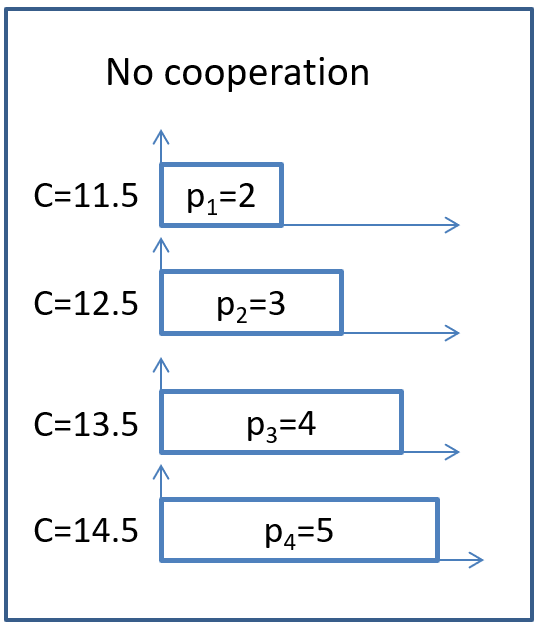
\includegraphics[width=1.1\textwidth]{Sche2.png}
  \end{figure}
  \end{column}

  \begin{column}{6.5cm}
  \vspace{-5mm}
  \begin{figure}[H]
  \centering
  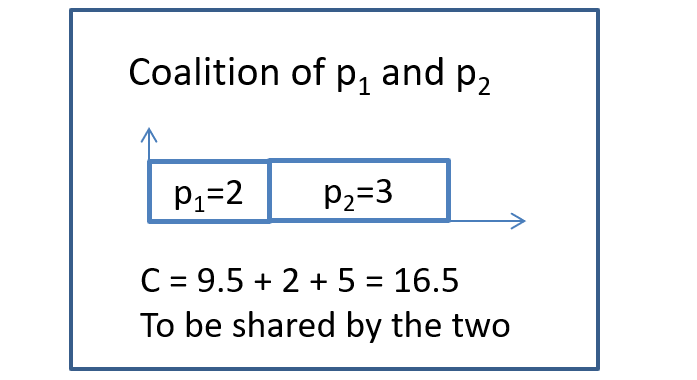
\includegraphics[width=1\textwidth]{Sche3.png}
  \end{figure}

  \vspace{-8mm}
  \begin{figure}[H]
  \centering
  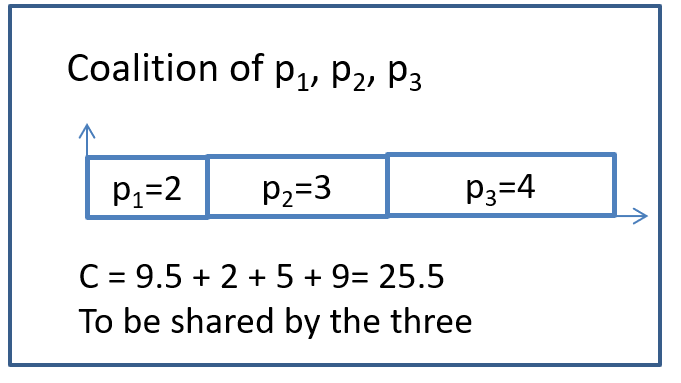
\includegraphics[width=6.2cm, height=3.1cm]{Sche4.png}
  \end{figure}

  \end{column}

  \end{columns}

\end{frame}


\begin{frame}{The Grand Coalition}

  \begin{figure}[H]
  \centering
  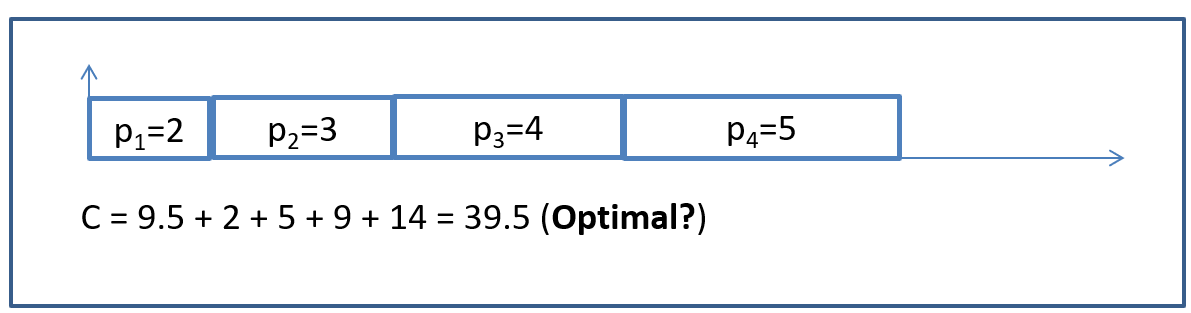
\includegraphics[width=1\textwidth]{Grand1.png}
  \end{figure}
  \centering

  \begin{figure}[htb]
  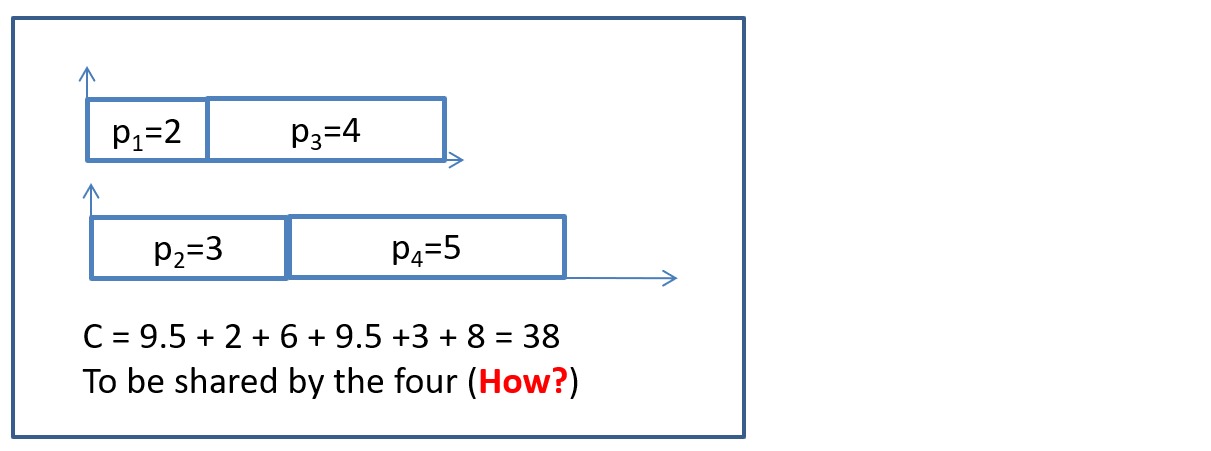
\includegraphics[width=1\textwidth]{Grand2.png}
  \end{figure}

\end{frame}


\begin{frame}{Related Concepts}
\begin{itemize}
\normalsize
\justifying
	\item Approximate core \\
  \vspace{0.25em}
  - ???
	\item Least core \\
  \vspace{0.25em}
  - ???
  \item $\ldots$\\
  \vspace{1em}
  \item Focusing on bounds
  \vspace{0.25em}
  \item How to help making decisions?

\end{itemize}
\end{frame}



\begin{frame}{Subsidization}
\small
\vspace{-4mm}
\begin{columns}

\begin{column}{6.5cm}
\footnotesize
\vspace{-1em}
\begin{shaded}
\centering
Optimal Cost Allocation Problem
\begin{eqnarray*}
\begin{aligned}
\max ~\big(\alpha_1 + \alpha_2 + \alpha_3 + \alpha_4\big) &= \textcolor{red}{37.25 < 38}\\
s.t.~~ \alpha_1 \leq 11.5,~\cdots,&~\alpha_4 \leq 14.5,\\
\alpha_1 + \alpha_2 \leq 16.5,~\cdots,~ &\alpha_3+\alpha_4 \leq 22.5,\\
~~~~~~~~~~\cdots,~~&\\
\alpha_1 + \alpha_2 + \alpha_3 + \alpha_4 &\leq 38.
\end{aligned}
\end{eqnarray*}
\vspace{-0.5em}
\end{shaded}
\begin{shaded}
\centering
\textcolor{blue}{
$\alpha^* = \big[6;8.75;10.75;11.75\big]$}
\end{shaded}
\end{column}

\begin{column}{4.5cm}
\small
\centering

\textcolor{red}{Subsidy}\\
\vspace{2em}
An outside party chips in $\omega=0.75$, making up the deficit.

\end{column}

\end{columns}
\end{frame}

\begin{frame}{Penalization}
\small
\vspace{-4mm}
\begin{columns}
\begin{column}{4.5cm}
\begin{table}[H]
\centering
\tabcolsep=8pt
\footnotesize
\renewcommand\arraystretch{1.1}
%\caption{\label{table:examplecost} Coalitional cost}
\vglue5pt
\vspace{-3mm}
\begin{tabular}[!h]{c c }
\hline
\multicolumn{1}{c}{Coalitions} &\multicolumn{1}{c}{Cost}\\
\hline
$\{1\}$		&11.5	\\

$\{2\}$		&12.5	\\

$\{3\}$		&13.5	\\

$\{4\}$		&14.5  \\

$\{1,2\}$		&16.5	\\

$\{1,3\}$		&17.5	\\

$\{1,4\}$		&18.5	\\

$\{2,3\}$		&19.5	\\

$\{2,4\}$		&20.5	\\

$\{3,4\}$		&22.5	\\

$\{1,2,3\}$		&25.5	\\

$\{1,2,4\}$		&26.5	\\

$\{1,3,4\}$		&28.5	\\

$\{2,3,4\}$		&31.5	\\

$\{1,2,3,4\}$	&38	\\
\hline
\end{tabular}
\end{table}
\end{column}
% \pause

\begin{column}{7cm}
\small
The outside party as the rule maker:\\
\vspace{1em}
\footnotesize
For any coalition that does not join the grand coalition, please pay a penalty of $z$.

\begin{shaded}
\vspace{-1.5em}
\begin{eqnarray*}
\begin{aligned}
\min z\\
s.t.~~ \alpha_1 \leq 11.5+z,~\cdots,&~\alpha_4 \leq 14.5+z,\\
\alpha_1 + \alpha_2 \leq 16.5+z,~\cdots,~ &\alpha_3+\alpha_4 \leq 22.5+z,\\
~~~~~~~~~~\cdots,~~&\\
\alpha_1 + \alpha_2 + \alpha_3 + \alpha_4 +\omega &\leq 38.
\end{aligned}
\end{eqnarray*}
\vspace{-1.5em}
\end{shaded}

\centering
$ Z_{\min}=0.5$ \\
\vspace{1em}
Result: No one pays the penalty

\end{column}
\end{columns}
\end{frame}

\begin{frame}{Simultaneous Subsidization and Penalization }
\small
\vspace{-4mm}
\begin{columns}
\begin{column}{4.5cm}
\begin{table}[H]
\centering
\tabcolsep=8pt
\footnotesize
\renewcommand\arraystretch{1.1}
%\caption{\label{table:examplecost} Coalitional cost}
\vglue5pt
\vspace{-3mm}
\begin{tabular}[!h]{c c }
\hline
\multicolumn{1}{c}{Coalitions} &\multicolumn{1}{c}{Cost}\\
\hline
$\{1\}$		&11.5	\\

$\{2\}$		&12.5	\\

$\{3\}$		&13.5	\\

$\{4\}$		&14.5  \\

$\{1,2\}$		&16.5	\\

$\{1,3\}$		&17.5	\\

$\{1,4\}$		&18.5	\\

$\{2,3\}$		&19.5	\\

$\{2,4\}$		&20.5	\\

$\{3,4\}$		&22.5	\\

$\{1,2,3\}$		&25.5	\\

$\{1,2,4\}$		&26.5	\\

$\{1,3,4\}$		&28.5	\\

$\{2,3,4\}$		&31.5	\\

$\{1,2,3,4\}$	&38	\\
\hline
\end{tabular}
\end{table}
\end{column}
% \pause

\begin{column}{7cm}
\small
\vspace{0.5em}
Outside party as the rule maker:\\
\vspace{1em}
\footnotesize
(1) For any coalition that does not join the grand coalition, please pay a penalty of $z$. \\
\vspace{0.5em}
(2) Outside party subsidizes grand coalition $\omega$.

\begin{shaded}
\vspace{-1.5em}
\begin{eqnarray*}
\begin{aligned}
% \max ~\big(\alpha_1 + \alpha_2 + \alpha_3 + \alpha_4\big) &= \textcolor{red}{37.25 < 38}\\
s.t.~~ \alpha_1 \leq 11.5+z,~\cdots,&~\alpha_4 \leq 14.5+z,\\
\alpha_1 + \alpha_2 \leq 16.5+z,~\cdots,~ &\alpha_3+\alpha_4 \leq 22.5+z,\\
~~~~~~~~~~\cdots,~~&\\
\alpha_1 + \alpha_2 + \alpha_3 + \alpha_4 +\omega &\leq 38.
\end{aligned}
\end{eqnarray*}
\vspace{-1.5em}
\end{shaded}

\centering

For example, $\omega= 1/2, z=1/6$

\end{column}
\end{columns}
\end{frame}

\end{document}
